\documentclass[
 aps,
 prd,
 reprint,
 superscriptaddress,
 nofootinbib,
 longbibliography
]{revtex4-2}

\usepackage{amsmath,amssymb}
\usepackage{booktabs}
\usepackage{graphicx}
\usepackage{mathrsfs}
\usepackage{capt-of}
\usepackage[hidelinks]{hyperref}
\hypersetup{
 pdftitle={Testing artificial cosmology as a regulator with Schwarzschild--de Sitter scalar waves},
 pdfauthor={Govind Arun Kumar and Anil Zenginoglu},
 pdfsubject={Curvature-coupled scalar-wave evolution on Schwarzschild--de Sitter and Schwarzschild spacetimes},
 pdfkeywords={general relativity, black holes, numerical relativity, null infinity, wave propagation, conformal coupling}
}

\newcommand{\scri}{\mathscr{I}}
\newcommand{\hc}{\mathcal{H}_{c}^{+}}
\newcommand{\hb}{\mathcal{H}_{b}^{+}}

\begin{document}

\title{Testing artificial cosmology as a regulator with
Schwarzschild--de Sitter scalar waves}

\author{Govind Arun Kumar}
\email{govind02@umd.edu}
\affiliation{Institute for Physical Science and Technology, University of
Maryland, College Park, Maryland 20742, USA}

\author{An\i l Zengino\u{g}lu}
\email[Corresponding author: ]{anil@umd.edu}
\affiliation{Institute for Physical Science and Technology, University of
Maryland, College Park, Maryland 20742, USA}

\date{\today}

\begin{abstract}
Conformal compactification of asymptotically flat evolution equations can
introduce formally singular terms at future null infinity.  Misner proposed
regulating them with a small positive cosmological constant, replacing null
infinity by a cosmological horizon where the conformal factor remains nonzero.
Using curvature-coupled scalar waves on Schwarzschild--de Sitter spacetime,
we test a necessary fixed-background benchmark for this proposal; we do not
test the regularity or conditioning of the conformal Einstein equations.  We
formulate both minimal coupling, $\xi=0$, and conformal coupling, $\xi=1/6$.
The former retains a curvature-dependent lower-order term after spacetime
compactification, whereas the latter is the scalar analogue of Misner's
conformally invariant Maxwell test.  A meaningful large-$L$
comparison requires the metric, foliation, compactification, initial-data map,
and waveform clock to approach a common Schwarzschild problem.  We construct
such a family with a bridge foliation and compare it with a separately evolved
Schwarzschild reference, which is shared by both couplings because the
Schwarzschild Ricci scalar vanishes.  The broad waveform and caustic production
suite uses $\xi=0$.  For $L/M=80,160,320,640$, direct waveform errors
decrease but depend on the observable.  Two nested extrapolants support
agreement with the Schwarzschild waveform within a conservative $1\%$ for the
cumulative, prompt-dominated pure-$\ell=2$ test through $U/M=160$ and for a
localized multimode $3+1$ response on the common interval
$0\lesssim U/M\leq57.2$.  This bound does not extend uniformly to late times.
For $\xi=0$, caustic-echo timing is consistent with local
$\mathcal O((M/L)^2)$ and outer
$\mathcal O(M/L)$ trends, although deterministic sensitivities preclude
precision fit coefficients.  These calculations test the fixed-background
feasibility of Misner's proposal.  For the same coupling, we also test a
static, spherically symmetric exterior-supported extension whose conserved
cosmological tensor vanishes in the strong-field region and reaches the
constant positive-$\Lambda$ form outside a smooth transition.  At fixed
exterior $\Lambda$, this construction improves the raw,
unshifted pure-$\ell=2$ QNM-window agreement with Schwarzschild.  Across
three fixed $30M$ windows, the relative error reduction ranges from
$20.9$--$30.2\%$ at $L/M=80$ to $7.8$--$9.3\%$ at $L/M=640$.
The fine-grid ordering clears conservative observed level-to-level margins at
every $L$.  The $L/M=640$ exterior ladder is nonmonotone and is not continuum
extrapolated.  The improvement remains modest at large $L$ and does not
determine the global quasinormal spectrum.
A matched $\ell=1$ outer-boundary study through $U/M=1000$ includes both
couplings.  Only uniform conformal SdS sustains a $142M$ intermediate interval
consistent with the Schwarzschild $U^{-3}$ Price law; uniform minimal SdS and
both exterior-supported cases fail the declared $40M$ persistence criterion.
The exterior signals instead contain convergent slow components and broad
secondary lobes associated with the altered exterior scattering problem.  Neither
uniform case resolves its expected asymptotic cosmological rate on the
evolved interval, and no asymptotic rate is assigned to the exterior family.
Application to the nonlinear Einstein equations motivates this work but lies
beyond its scope.
\end{abstract}

\maketitle

%%%%%%%%%%%%%%%%%%%%%%%%%%%%%%%%%%%%%%%%%%%%%%%%%%%%%%%%%%%%%%%%%%%%%%%%%%%%%%%
\section{Introduction}
\label{sec:introduction}
%%%%%%%%%%%%%%%%%%%%%%%%%%%%%%%%%%%%%%%%%%%%%%%%%%%%%%%%%%%%%%%%%%%%%%%%%%%%%%%

Radiation from isolated systems has a clean definition at future null
infinity, $\scri^+$.  Hyperboloidal evolution brings this boundary onto the
computational domain through spacelike slices that approach
outgoing null hypersurfaces.  After spatial compactification places infinity
at a finite coordinate location, waves leave the grid through a
characteristic, pure-outflow boundary.  Several programs have pursued this
goal for the nonlinear Einstein equations.  Characteristic evolution and
Cauchy--characteristic matching form a complementary line of work
\cite{Winicour:2012characteristic}.  Recent work applied matching to nine
fully nonlinear binary-black-hole merger simulations and used it to resolve
late-time tails \cite{MaEtAl:2025CCM}.

Two conformal-field-equation programs avoid directly evolving the formally
singular conformally rescaled metric equations by enlarging the regular
variable set.  Friedrich's conformal field equations give a first-order
formulation \cite{friedrich1983cauchy}; early
implementations evolved weak radiative data in three dimensions through
regular future timelike infinity and isolated systems in axisymmetry
\cite{Frauendiener:1998II,Hubner:1999scheme,Hubner:2001timelike,
FrauendienerHein:2002}.  They also exposed the costs: many variables and
constraints, delicate initial data, and gauge sensitivity.  In standard early
reductions, $\scri^+$ was an inward-moving null hypersurface ending at
$i^+$ unless a gauge froze its coordinate location.  As $\scri^+$ crossed the
grid, the coordinate region representing the physical spacetime contracted
and progressively lost resolution, which obstructed accurate long-time
waveform evolution \cite{Husa:2002problems}.  Friedrich's generalized
equations instead use a Weyl connection and conformal geodesics
\cite{Friedrich:1995general,Friedrich:2003geodesics}.  In conformal Gauss
gauge, the initial gauge data determine the conformal factor explicitly.  The
method has enabled nonlinear black-hole scattering from past to future null
infinity \cite{BeyerEtAl:2017GCFE,FrauendienerStevens:2021massloss,
FrauendienerStevensThwala:2025}.  The current initial-boundary framework
does not keep $\scri^+$ at a fixed outer spatial coordinate
\cite{CamdenEtAl:2025}, and conformal-Gauss compactification can degrade
resolution in physical time at late times
\cite{FrauendienerStevens:2023compactification}.

Scri fixing removes this particular loss mechanism by holding $\scri^+$ at a
fixed spatial boundary.  On fixed black-hole backgrounds it also places the
event horizon and $\scri^+$ at characteristic outflow boundaries, eliminates
artificial outer boundary data and finite-radius waveform extrapolation, and
leaves a time-independent compact domain
\cite{zenginoglu_hyperboloidal_2008,Zenginoglu:2008pw}.  Time-domain
black-hole perturbation calculations established the accuracy and efficiency
of this gauge for Schwarzschild and Kerr, including direct waveforms for
mass-ratio systems and long evolutions that resolve power-law tails at
$\scri^+$
\cite{zengin2008hyperboloidal,ZenginogluNunezHusa:2009,
ZenginogluTiglio:2009,RaczToth:2011,Bernuzzi:2011aj,
ZenginogluKhanna:2011,Harms:2014dqa}.  Frequency-domain formulations later
used the same horizon-to-$\scri^+$ regularity to avoid asymptotic boundary
conditions and to build accurate spectral decompositions and efficient
self-force solvers
\cite{AnsorgMacedo:2016,Macedo:2020,MacedoEtAl:2022}.  These results motivate
our standpoint: scri fixing is a desirable numerical gauge, not merely a
choice of compactifying coordinates.  The finite-$L$ family below preserves
this fixed-endpoint structure and approaches a scri-fixed Schwarzschild gauge
as $L\to\infty$.  A complementary hyperboloidal treatment implements
Geroch's limiting procedure for the Schwarzschild, de Sitter, and Nariai
limits of the SdS family \cite{ZhouPanossoMacedo:2025}.

Model fields also allow asymptotic formulations to be tested in full $3+1$
codes before they are used for the Einstein equations.  An early calculation
evolved nonsymmetric scalar data on Minkowski and Schwarzschild backgrounds
with $\scri^+$ as a fixed outflow boundary \cite{ZenginogluKidder:2010}.
Recent work has evolved three-dimensional nonlinear wave models on
compactified Minkowski hyperboloids without imposing symmetry
\cite{Peterson:2023bha,Rinne:2025nonlinear,
ZenginogluBernuzziNutzi:2026}.  This calculation complements those
tests with a fully angle-dependent $3+1$ scalar field on black-hole
backgrounds: the outer boundary is the cosmological horizon at finite $L$ and
$\scri^+$ for the separately evolved Schwarzschild reference.  A
spherical-harmonic representation tests angular truncation, multimode
reconstruction, caustic interference, and the characteristic spherical outer
boundary, while the symmetry of the background permits an exact reduction to
independent radial mode equations.  This reduction is an optimization
specific to this linear spherical problem, not a restriction of the numerical
infrastructure to $1+1$ fields.  The angular transforms, modal representation,
time integration, and boundary machinery form $3+1$ infrastructure intended
for coupled nonlinear fields and nonspherical backgrounds such as Kerr.  Those
applications would replace the diagonal radial evolution by a coupled
evolution operator; they are prospective and are not tested here.

The corresponding prescribed-factor metric equations retain familiar
evolution variables and obtain finite limits of formally singular terms from
the constraints and conformal gauge
\cite{zenginoglu_hyperboloidal_2008,Zenginoglu:2008pw}.  Nonlinear conformal
BSSN/Z4 demonstrations remain spherical: self-gravitating scalar fields
\cite{Vano-Vinuales:2014koa,Vano-Vinuales:2017qij}, vacuum Minkowski
reference-metric and layer tests \cite{VanoVinuales:2024reference}, and
charged Einstein--Maxwell--Klein--Gordon collapse \cite{Alvares:2025emkg}.
A constrained CMC route instead derives regular boundary values from the
constraints and shear-free condition \cite{Moncrief:2008ie}.  It has produced
twist-free axisymmetric vacuum evolutions with Bondi news at fixed $\scri^+$
\cite{Rinne:2009qx} and spherical Einstein--matter evolutions
\cite{RinneMoncrief:2013}.  Three-dimensional CMC black-hole initial data and
a general constrained tetrad formulation also exist
\cite{BuchmanPfeifferBardeen:2009,BardeenSarbachBuchman:2011}, but the
dynamical vacuum evolutions have so far reached only twist-free axisymmetry,
and the approach's elliptic sector is not yet integrated with generic
binary-black-hole free evolution.

Dual-foliation generalized harmonic evolution separates strong-field
coordinates from a compactified hyperboloidal target system.  Its formulation
and three-dimensional flat-space scalar tests established the construction
\cite{Hilditch:2015aba,HilditchEtAl:2018}; later gauge and constraint additions
controlled logarithms and formally singular terms \cite{DuarteEtAl:2023}.
The program has since advanced to full Einstein evolution in spherical
symmetry \cite{Peterson:2024spherical,Peterson:2025strong}.  The
full-Einstein demonstrations are therefore still spherical and contain no
radiative gravitational degree of freedom.  Separately, N\"utzi constructed a
quasilinear symmetric-hyperbolic vacuum system about Minkowski spacetime with
fixed null infinity
\cite{Nutzi:2023,Nutzi:2025}, together with compatible nonlinear constraint
solutions \cite{Nutzi:2026}.  This genuinely nonlinear result remains
analytical and restricted to small data; it does not yet cover a generic
strong-field interior.

To our knowledge, a robust, generic three-dimensional metric free-evolution
code that fixes $\scri^+$ at the outer boundary while supporting binary black
holes remains to be demonstrated.  Misner's artificial cosmology
\cite{misner_hyperboloidal_2006,misner_over_2006,misner_excising_2006} is
closest in spirit to prescribed-factor evolution, but replaces the
$\Omega_0=0$ endpoint by a cosmological horizon where
$\Omega_L=r_b/r_c>0$.  It thereby trades the direct conformal limit for a
finite-$L$ physical bias and an extrapolation problem.  This scalar model
measures that bias and tests the extrapolation; only a nonlinear Einstein
evolution can determine whether it improves regularity, constraint behavior,
and conditioning.
At finite $L$, the cosmological horizon provides a characteristic outer
boundary; the grid may end there, as ours does, or extend into a pure-outflow
region.  The black-hole horizon similarly supports inner excision.  Misner
and collaborators tested the idea with Maxwell fields on de Sitter
backgrounds, choosing a conformally invariant system so that the dropped
spacetime conformal factor did not enter the field equations.  The
curvature-coupled scalar family
\begin{equation}
 (\Box-\xi R)\Phi=0
 \label{eq:intro_curvature_coupling}
\end{equation}
contains both a conventional minimally coupled test field ($\xi=0$) and the
scalar conformal analogue ($\xi=1/6$).  Brady et al. analyzed the same family
for general $\xi$, including these two cases
\cite{brady_radiative_1999}.  Formulating both here allows us to distinguish
coupling-independent regulator behavior from sensitivity to the asymptotic
field equation.
Scalar waves on Schwarzschild--de Sitter (SdS) provide a black-hole model with a
strong-field scattering region between the future black-hole horizon $\hb$
and the future cosmological horizon $\hc$.

For $\Lambda>0$, the future conformal boundary is spacelike.  Its asymptotic
symmetries and radiative degrees of freedom differ from those at
$\scri^+$, as do the associated fluxes.  Ashtekar et al. developed this
structure for linear fields and derived a
positive-$\Lambda$ quadrupole formula
\cite{Ashtekar:2014zfa,Ashtekar:2015lla,Ashtekar:2015lxa}.  Here we study
only the finite-$L$ bias and large-$L$ limit of scalar evolution on fixed
backgrounds.  We determine the region over which that evolution approximates
a specified asymptotically flat solution, with the cosmological horizon
confining the comparison to a finite spacetime region.

Regularity at $\hb$ and $\hc$ fixes the leading behavior of a bridge near
each horizon.  Its continuation into the expanding region beyond $\hc$
selects the asymptotic end.  Horizon crossings leave enough freedom for a
one-parameter family to approach a Cauchy-like Schwarzschild end.  The
candidate artificial-cosmology family includes its foliation and
compactification along with the data map and waveform clock.  Scalar
observables remain invariant under coordinate changes.  Our analysis tracks
the limiting coordinates and the conditioning they induce in the scalar
evolution equations.

Writing $\Lambda=3/L^2$, the SdS metric approaches Schwarzschild on every
fixed near-zone interval as $L/M\to\infty$.  Each finite value of $L$ keeps
the SdS global causal structure.  Schwarzschild fields develop inverse-power
tails
\cite{price1972nonspherical,zengin2008hyperboloidal,
Angelopoulos:2016wcv}.  SdS fields eventually display cosmological decay
whose rate depends on $\xi$
\cite{Brady:1996za,brady_radiative_1999,Molina:2003dc}.  In the large-horizon
limit, Brady et al. find the decay rate
\begin{equation}
 \frac{\gamma_{\ell,\xi}}{\kappa_c}
 =\ell+\frac32-\frac12\sqrt{9-48\xi}
 +\mathcal O(M/L),
 \label{eq:intro_brady_exponent}
\end{equation}
so the leading $\ell=1$ values are
$\gamma_{1,0}/\kappa_c=1$ and
$\gamma_{1,1/6}/\kappa_c=2$.
A finite-$L$
calculation approximates the asymptotically flat waveform over a finite
interval.  Cosmological decay sets its later behavior.

Using the bridge constructions and conformal geometry developed in
Ref.~\cite{zenginoglu_bridge_2025}, we form a one-parameter family of
candidate artificial-cosmology backgrounds on a fixed compact domain.
Analytic large-$L$ limits follow the slices to their asymptotic ends.
Retarded-time offsets set a common clock, and the compactified coefficients
expose the conditioning of each choice.  The broad production suite evolves
the $\xi=0$ system in the minimal gauge and compares each finite-$L$ waveform
with a separately evolved Schwarzschild reference without fitting a relative
time translation.  The dedicated outer-boundary tail experiment also evolves
the matched $\xi=1/6$ comparator.  Only the lower-order potential changes:
the foliation, characteristic speeds, data map, and Schwarzschild reference
are common.

Five logically distinct questions should be separated.  First, can one
construct a finite-$L$ metric, foliation, and compactification with a global
Schwarzschild limit?  Second, do matched observables admit useful direct or
extrapolated recovery as $L\to\infty$?  Third, can exterior support improve
that recovery at the same exterior $\Lambda$?  Fourth, which conclusions are
robust under the change from minimal to conformal scalar coupling?  Fifth,
does finite $L$ actually
regularize and condition the formally singular terms in a nonlinear conformal
Einstein evolution?  This paper answers the first two questions on fixed
black-hole backgrounds using scalar waves and tests the third with a
pure-$\ell=2$ waveform.  The quantitative evidence for those tests uses
$\xi=0$.  We test the fourth question in the matched $\ell=1$ tail sector;
the broader fixed-mode, localized-source, and caustic results remain
minimally coupled.
The exterior-supported geometry uses a conserved
cosmological tensor and fixed nonzero Chebyshev-angle widths for both its
transition and exact-SdS cap.  Section~\ref{sec:exterior-tests} gives the
corresponding numerical comparison.  The fifth question requires a
nonlinear Einstein evolution code and is left for future work.

Misner's uniform-$\Lambda$ sequence distributes its finite-$L$ bias throughout
the static patch, including the strong-field and wave-generation regions.  The
direct comparisons below consequently require $L/M$ of several hundred for
percent-level prompt-waveform agreement.  As a further improvement upon his
suggestion, we consider, within a static spherical model, an
exterior-supported cosmological tensor that leaves the near zone exactly
Schwarzschild and confines the modification to a smooth outer layer.  This
trade may permit smaller
$L/M$ while preserving prompt strong-field observables.  Equivalently, at
the same exterior $\Lambda$ the exterior-supported waveform may approximate the
Schwarzschild waveform more closely than uniform SdS.  This fixed-background
conjecture is the central test of the extension; the layer can scatter waves
and alter the global spectrum, so the conjecture cannot be inferred from the
exact near-zone geometry.

Within that scope, the primary goal is to quantify the direct finite-$L$
error and the accuracy of an $L\to\infty$ scalar-wave extrapolation for
$\xi=0$.  A fixed pure-$\ell=2$ datum tests the waveform limit cleanly, while
a localized source excites many angular modes and probes the construction
through caustics.  A supporting physics goal is to study finite-$\Lambda$
effects, including caustic echoes and departure from Schwarzschild late-time
behavior.  The matched $\ell=1$ tail experiment then tests sensitivity to
conformal coupling; no coupling comparison is made for the broader fixed-mode,
localized-source, caustic, or exterior-QNM suites.

Section~\ref{sec:bridges} gives the global foliation criterion and identifies
the benchmark gauge.  Section~\ref{sec:scalar} defines the scalar model,
matched data, clock, numerical methods, and comparison measures.
Section~\ref{sec:results} gives direct and extrapolated Schwarzschild
recovery followed by the localized-source test and supporting SdS physics.
Section~\ref{sec:exterior-supported} constructs a fixed-angle-width
exterior-supported extension and reports both the short $\xi=0$ waveform
comparison and the matched tail result.  The appendices collect convergence,
sensitivity, and reproducibility details.

%%%%%%%%%%%%%%%%%%%%%%%%%%%%%%%%%%%%%%%%%%%%%%%%%%%%%%%%%%%%%%%%%%%%%%%%%%%%%%%
\section{Bridge foliations and the scalar-wave
large-\texorpdfstring{$L$}{L} limit}
\label{sec:bridges}
%%%%%%%%%%%%%%%%%%%%%%%%%%%%%%%%%%%%%%%%%%%%%%%%%%%%%%%%%%%%%%%%%%%%%%%%%%%%%%%

\subsection{Schwarzschild--de Sitter static patch}

The SdS metric in static coordinates is
\begin{align}
 ds^2&=-f(r)dt^2+\frac{dr^2}{f(r)}+r^2d\omega^2,
 \label{eq:sds_metric}\\
 f(r)&=1-\frac{2M}{r}-\frac{r^2}{L^2},
 \qquad d\omega^2=d\theta^2+\sin^2\theta\,d\varphi^2.
 \label{eq:f}
\end{align}
We use geometrized units $G_{\rm N}=c=1$.  The simulations set $M=1$;
coordinates are quoted in units of $M$, and comparison measures are
dimensionless.
For $0<M<L/(3\sqrt{3})$, $f$ has a black-hole root $r_b$, a
cosmological root $r_c$, and a negative root $r_u=-(r_b+r_c)$.  They obey
\begin{align}
 L^2&=r_b^2+r_br_c+r_c^2,
 &2ML^2&=r_br_c(r_b+r_c),
 \label{eq:root_relations}\\
 f(r)&=\frac{(r-r_b)(r_c-r)(r-r_u)}{L^2r}.
 \label{eq:f_factorized}
\end{align}
For $i=b,c$, the positive surface gravities follow from
Eq.~\eqref{eq:kappa}.  The partial-fraction formulas use the positive
algebraic coefficient $\kappa_u:=|f'(r_u)|/2$ at the negative root:
\begin{equation}
 \kappa_i=\frac12\left|f'(r_i)\right|
 =\frac12\left|\frac{1}{r_i}-\frac{3r_i}{L^2}\right|,
 \qquad i\in\{b,c,u\}.
 \label{eq:kappa}
\end{equation}
With an arbitrary reference radius $r_0\in(r_b,r_c)$, the normalized
tortoise coordinate is
\begin{align}
r_{*,L}(r)={}&\frac{1}{2\kappa_b}
 \ln\frac{r-r_b}{r_0-r_b}
-\frac{1}{2\kappa_c}
 \ln\frac{r_c-r}{r_c-r_0}
\notag\\
&+\frac{1}{2\kappa_u}
 \ln\frac{r-r_u}{r_0-r_u}.
\label{eq:tortoise}
\end{align}
The tortoise coordinate tends to $-\infty$ at $r_b$ and to $+\infty$ at
$r_c$.  Its flat limit has
\begin{equation}
 r_b\to2M,\qquad r_c=L-M+\mathcal{O}(M^2/L),
 \label{eq:horizon_flat_limit}
\end{equation}
and the static patch expands to the Schwarzschild exterior.
The geometric identification needed to make this Schwarzschild limit precise
is discussed in Ref.~\cite{ZhouPanossoMacedo:2025}.

\subsection{The global criterion beyond the horizons}

We introduce a stationary height function,
\begin{equation}
 \tau=t+h(r),\qquad B(r):=f(r)h'(r),
 \label{eq:height}
\end{equation}
where $B$ is the boost relative to $r_*$.  For a radial coordinate
$\rho=g(r)$ and $G=d\rho/dr$, the metric becomes
\begin{equation}
 ds^2=-f\,d\tau^2+\frac{2B}{G}\,d\tau d\rho
 +\frac{1-B^2}{fG^2}\,d\rho^2+r^2d\omega^2.
 \label{eq:transformed_metric}
\end{equation}
A future-directed spacelike bridge within the static patch satisfies
\begin{equation}
 |B|<1,\qquad B(r_b)=+1,\qquad B(r_c)=-1,
\label{eq:boost_conditions}
\end{equation}
where $(1-B^2)/f$ must tend to a finite positive nonzero value at each
horizon for a radial map with finite nonzero endpoint values of $G$.
Equivalently, $h\sim+r_*$ at $\hb$ and $h\sim-r_*$ at $\hc$.  The leaves
are null-transverse and the transformed coefficients have regular horizon
limits \cite{zenginoglu_bridge_2025}.  Beyond $\hc$, where $f<0$, spacelike
continuation on the future branch requires $B<-1$.  The value $B(r_c)=-1$
supplies the local crossing data.  The behavior of $B$ beyond that point
determines how the leaves approach the spacelike future boundary.  This
expanding region supports forward and scattering problems
\cite{Schlue:2012pq,Bernhardt:2024hfs}.

Two heights normalized by $h(r_0)=0$ carry the same endpoint data:
\begin{align}
h_{\rm min}(r)={}&
\frac{1}{2\kappa_b}\ln\left|\frac{r-r_b}{r_0-r_b}\right|
+\frac{1}{2\kappa_c}\ln\left|\frac{r_c-r}{r_c-r_0}\right|,
\label{eq:minimum_height}\\
h_{\rm mg}(r)={}&
\frac{1}{2\kappa_b}
\ln\left|\frac{(r-r_b)r_0}{(r_0-r_b)r}\right|
+\frac{1}{2\kappa_c}
\ln\left|\frac{(r_c-r)r_0}{(r_c-r_0)r}\right|
\notag\\
&-\frac{1}{2\kappa_u}
\ln\left|\frac{(r-r_u)r_0}{(r_0-r_u)r}\right|.
\label{eq:minimal_height}
\end{align}
Local horizon regularity supplies the two logarithms in the minimum height.
The construction underlying the minimal gauge was developed for
hyperboloidal QNM expansions
\cite{AnsorgMacedo:2016,MacedoJaramilloAnsorg:2018} and named in
Ref.~\cite{Macedo:2020}.  Its derivation for static spherical metrics uses the
in--out and out--in strategies of Ref.~\cite{PanossoMacedo:2023qzp}.  For SdS,
the out--in construction adds the regular third-root contribution and yields a
controlled Schwarzschild limit \cite{ZhouPanossoMacedo:2025}.
Equation~\eqref{eq:minimal_height} is that construction in our sign and
normalization conventions.  Equation
\eqref{eq:boost_conditions} holds for both families.  Figure
\ref{fig:bridge_foliations} follows their leaves beyond $\hc$.  As
$L\to\infty$, the minimum-height family closes toward a Cauchy-like
asymptotic end.  Minimal-gauge leaves open toward Schwarzschild $\scri^+$,
as seen in the two conformal diagrams.

\begin{figure*}[t]
 \centering
 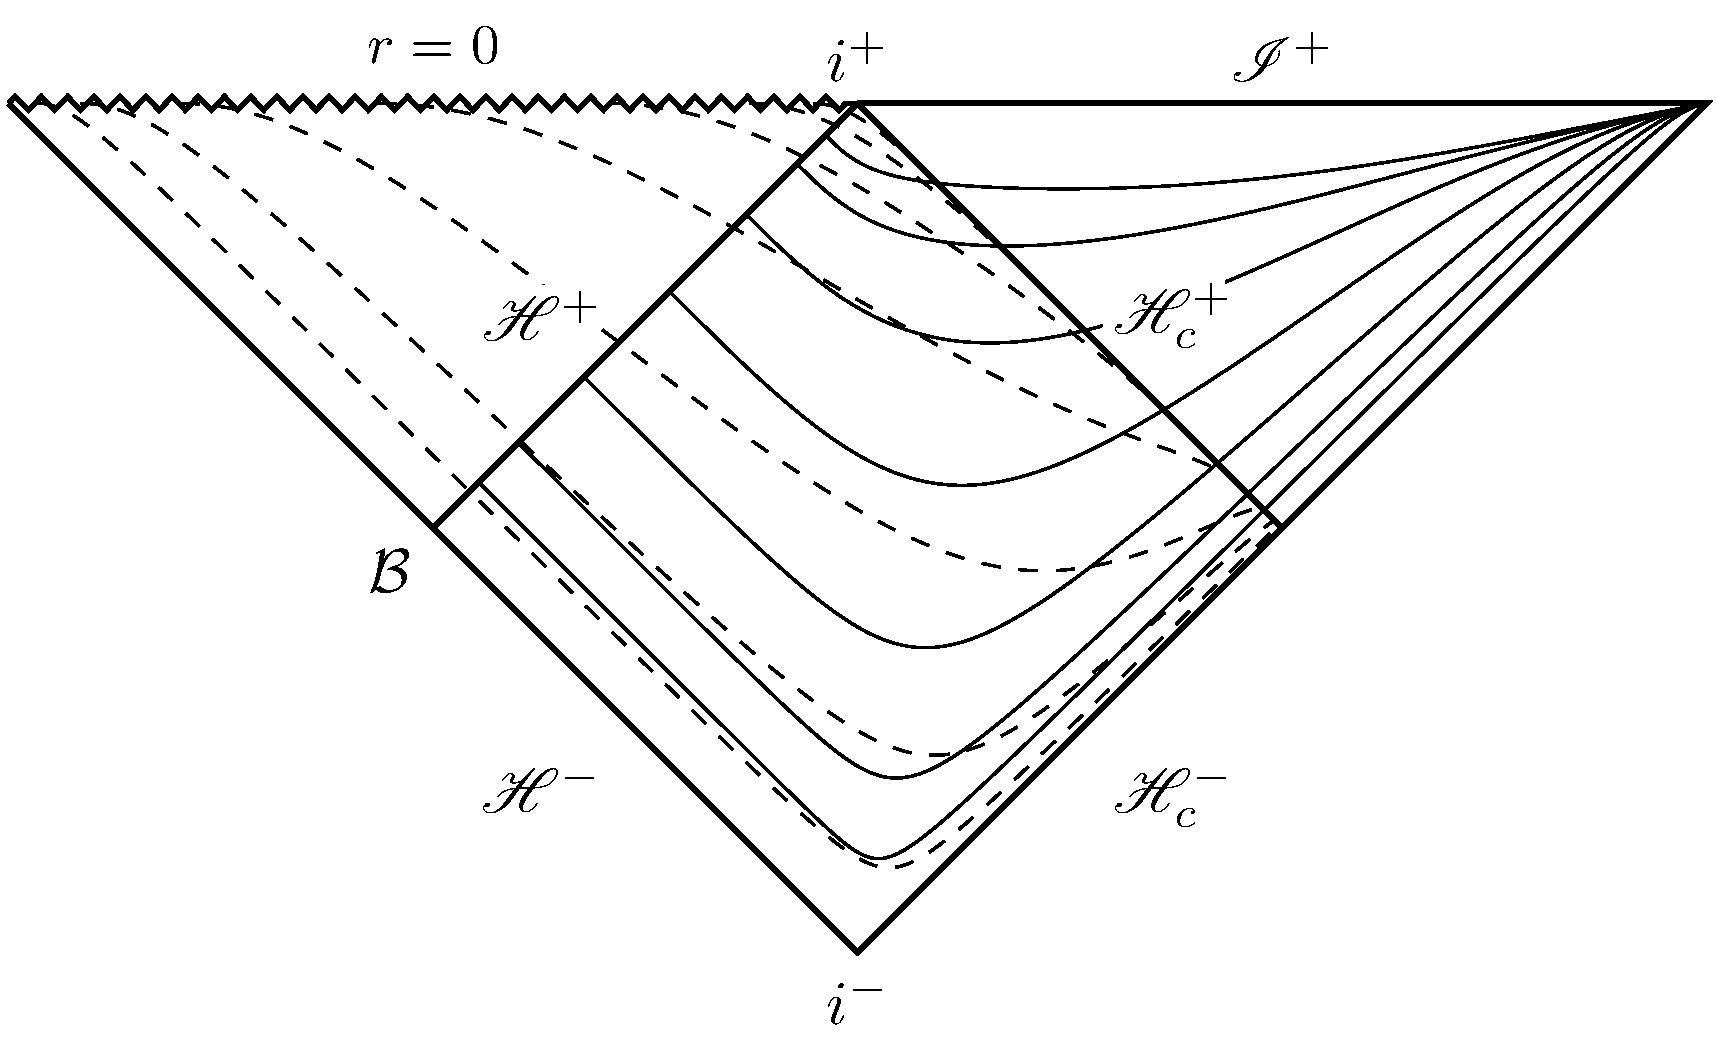
\includegraphics[width=0.49\textwidth]{figs/minimalAnil.pdf}
 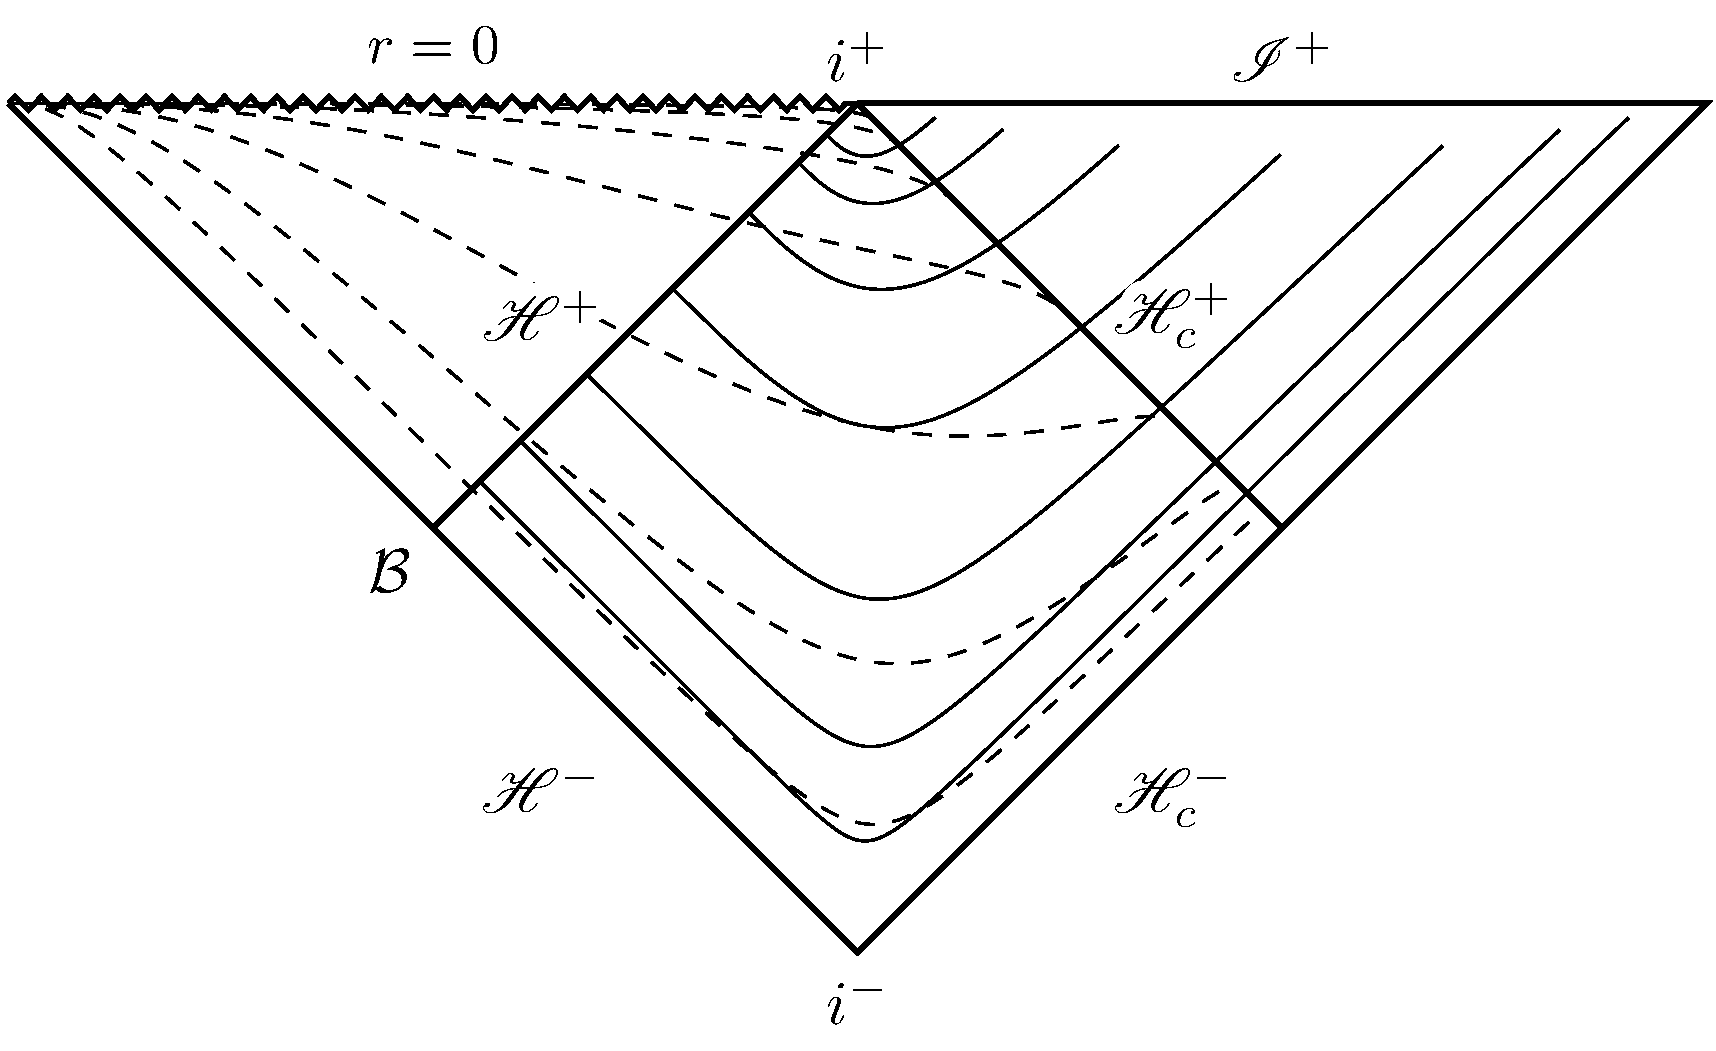
\includegraphics[width=0.49\textwidth]{figs/minimalRodrigo.pdf}
 \caption{Conformal diagrams of two SdS bridge families.  Each family crosses the
 future horizons regularly.  The minimum-height leaves
 in the left panel close toward a Cauchy-like end as $L$ grows.  In the
 right panel, minimal-gauge leaves open toward Schwarzschild $\scri^+$.
 Solid and dashed curves belong to the separate horizon-regular conformal
 charts used to construct the diagrams.  Adapted from
 Ref.~\cite{zenginoglu_bridge_2025} under the
 \href{https://creativecommons.org/licenses/by/4.0/}{Creative Commons
 Attribution 4.0 International License}.}
 \label{fig:bridge_foliations}
\end{figure*}

For a bridge normalized by $h(r_0)=0$ and $r_{*,L}(r_0)=0$, the boost gives
the clock diagnostic
\begin{equation}
 q_B(L;r_0):=\lim_{r\to r_c}(h+r_{*,L})
 =\int_{r_0}^{r_c}\frac{1+B}{f}\,dr.
 \label{eq:general_q}
\end{equation}
The integrand is regular at $r_c$.  A divergent $q_B$ sends the origin of
the source clock to infinity as the outer null surface recedes.  A finite
$q_B$ supplies the required clock limit.

\subsection{Six bridges and a fixed compactification}

In addition to Eqs.~\eqref{eq:minimum_height} and
\eqref{eq:minimal_height}, we consider four boosts specified directly:
\begin{align}
B_{\rm lin}&=-1+2\frac{r_c-r}{r_c-r_b},
\label{eq:linear_boost}\\
B_{\rm fl}&=-1+2\frac{r_c-r}{r_c-r_b}\frac{r_b^2}{r^2},
\label{eq:flat_linear_boost}\\
B_{\rm Mav}&=-\frac{1-3M/r}{\sqrt{1-9M^2\Lambda}}
 \sqrt{1+\frac{6M}{r}},
\label{eq:mav_boost}\\
B_{\rm sr}&=-\gamma r+\frac{\beta}{r^2},
\label{eq:slow_roll_boost}\\
\gamma&=\frac{r_c^2+r_b^2}{r_c^3-r_b^3},\qquad
\beta=\frac{r_c^2r_b^2(r_c+r_b)}{r_c^3-r_b^3}.
\label{eq:slow_roll_parameters}
\end{align}
The Mavrogiannis boost is motivated by wave estimates on SdS and turns at the
photon sphere $r=3M$
\cite{mavrogiannis2024quasilinear,mavrogiannis2023morawetz}.

At fixed areal radius, with $x=M/r$, the six boosts have the limits
\begin{equation}
\begin{array}{lcc}
\text{bridge}&B_0(r)&B_0(\infty)\\
\hline
\text{minimum height}&3x-\tfrac12&-\tfrac12\\
\text{minimal gauge}&-1+8x^2&-1\\
\text{linear}&+1&+1\\
\text{modified linear}&-1+8x^2&-1\\
\text{Mavrogiannis}&-(1-3x)\sqrt{1+6x}&-1\\
\text{slow roll}&4x^2&0
\end{array}
\label{eq:boost_limits}
\end{equation}
An outgoing Schwarzschild hyperboloidal slice necessarily has $B_0\to-1$ at
$r\to\infty$.  With the compactification \eqref{eq:compactification}, a
regular null-infinity limit further requires
$1+B_0=\mathcal{O}(M^2/r^2)$ with a finite positive leading coefficient.
The minimum-height, linear, and slow-roll limits fall outside this
asymptotic-nullness condition.  Minimal, modified-linear, and Mavrogiannis
slices satisfy it.  A globally consistent scalar-wave comparison also
requires uniform compactified coefficients through the expanding region.
For the modified-linear boost, an outer layer breaks uniformity near
$\rho=1$.

We place both horizons at fixed coordinate locations using
\begin{align}
 \rho&=\frac{1-r_b/r}{1-r_b/r_c},
 &r(\rho)&=\frac{r_b}{1-(1-r_b/r_c)\rho},
 \label{eq:compactification}\\
 G(r)&=\frac{d\rho}{dr}
 =\frac{r_b}{(1-r_b/r_c)r^2}.
 \label{eq:G}
\end{align}
The black-hole and cosmological horizons are at $\rho=0$ and $1$,
respectively.  At fixed $r$,
\begin{equation}
 \rho\to\rho_0:=1-\frac{2M}{r},
 \label{eq:rho_limit}
\end{equation}
which is also the compactification used by the separate Schwarzschild
implementation.

The corresponding dimensionless spacetime conformal factor may be chosen as
\begin{equation}
 \Omega_L:=\frac{r_b}{r}
 =1-\left(1-\frac{r_b}{r_c}\right)\rho .
 \label{eq:conformal_factor}
\end{equation}
At every finite $L$ the outer endpoint is the cosmological horizon and
\begin{equation}
 \Omega_L(1)=\frac{r_b}{r_c}>0.
 \label{eq:finite_L_conformal_factor}
\end{equation}
In the Schwarzschild limit,
$\Omega_L\to\Omega_0=1-\rho$ and $\Omega_0(1)=0$, so the same endpoint becomes
$\scri^+$.  Equation~\eqref{eq:finite_L_conformal_factor} is the geometric
premise of the regulator mechanism in Misner's proposal: in a finite-$L$
Einstein problem, factors that become formally singular when $\Omega_0=0$
would instead be evaluated at nonzero $\Omega_L$.  Nonvanishing $\Omega_L$
alone does not establish regularity or good conditioning as $L$ grows.  The
scalar equations contain neither the tensorial conformal Einstein source
terms nor their gauge and constraint couplings and therefore cannot test
their regularization.  The relevant scaling can nevertheless be seen
schematically.  If $g$ satisfies $G_{ab}[g]+\Lambda g_{ab}=0$ and
$\bar g=\Omega_L^2g$, then
\begin{equation}
 G_{ab}[\bar g]=\mathcal T_{ab}[\Omega_L]
 -\frac{\Lambda}{\Omega_L^2}\bar g_{ab},
 \label{eq:conformal_einstein_scaling}
\end{equation}
where $\mathcal T_{ab}$ collects derivatives of $\Omega_L$
\cite{Zenginoglu:2008pw}.  At the cosmological horizon,
$\Lambda/\Omega_L^2\to3/(4M^2)$ as $L/M\to\infty$.  Minimal scalar coupling
retains a lower-order endpoint contribution with the same
$\Lambda/\Omega_L^2$ scaling, whereas conformal coupling cancels it.  The two
cases thus provide an algebraic stress test and a conformally regular
radiative analogue, respectively, without serving as surrogates for the
Einstein system.  Both test whether matched scalar observables on this
background and foliation family recover their Schwarzschild counterparts in
a controlled large-$L$ limit.

%%%%%%%%%%%%%%%%%%%%%%%%%%%%%%%%%%%%%%%%%%%%%%%%%%%%%%%%%%%%%%%%%%%%%%%%%%%%%%%
\section{Scalar evolution and comparison protocol}
\label{sec:scalar}
%%%%%%%%%%%%%%%%%%%%%%%%%%%%%%%%%%%%%%%%%%%%%%%%%%%%%%%%%%%%%%%%%%%%%%%%%%%%%%%

\subsection{Curvature coupling and regular first-order system}

We study the massless curvature-coupled equation
\begin{equation}
 \left(\Box_g-\xi R[g]\right)\Phi=0,
 \qquad \xi\in\left\{0,\frac16\right\},
 \label{eq:curvature_coupled_wave}
\end{equation}
where $g$ denotes the physical SdS or Schwarzschild metric.  Minimal coupling
has $\xi=0$; conformal coupling in four spacetime dimensions has $\xi=1/6$.
Write
\begin{equation}
 \Phi(t,r,\theta,\varphi)=\frac{1}{r}
 \sum_{\ell m}u_{\ell m}(t,r)Y_{\ell m}(\theta,\varphi).
 \label{eq:scalar_decomposition}
\end{equation}
Each mode satisfies
\begin{align}
 \left(-\partial_t^2+\partial_{r_*}^2-V_{\ell,\xi}\right)u&=0,
 \label{eq:wave_equation}\\
 V_{\ell,\xi}&=f\left[\frac{\ell(\ell+1)}{r^2}
 +\frac{f'(r)}{r}+\xi R[g]\right].
 \label{eq:scalar_potential}
\end{align}
For uniform SdS, $R[g]=12/L^2$ and therefore
\begin{equation}
 V_{\ell,\xi}=f\left[\frac{\ell(\ell+1)}{r^2}
 +\frac{2M}{r^3}+\frac{2(6\xi-1)}{L^2}\right].
 \label{eq:uniform_coupled_potential}
\end{equation}
The explicit $-2/L^2$ term occurs at $\xi=0$ and cancels at $\xi=1/6$.
In Schwarzschild, $R[g]=0$, so both couplings give the same equation and the
same reference waveform.

The relation to the spacetime compactification is instructive.  Let
$\bar g=\Omega_L^2 g$ and $\phi=\Omega_L^{-1}\Phi$.  For the sourced equation,
conformal covariance gives the single identity
\cite{ZenginogluKidder:2010}
\begin{equation}
 \left(\Box_{\bar g}-\frac{R[\bar g]}6\right)\phi
 +\left(\frac16-\xi\right)\frac{R[g]}{\Omega_L^2}\phi
 =\Omega_L^{-3}S.
 \label{eq:conformal_source_transform}
\end{equation}
The second term remains for $\xi=0$ and vanishes for $\xi=1/6$.  Since
$\Omega_L=r_b/r$, each evolved modal field is proportional to its unphysical
counterpart, $\phi_{\ell m}=(u_{\ell m}/r_b)Y_{\ell m}$.  Thus the distinction is not
whether the evolved variable is rescaled; it is which physical curvature
coupling that variable represents.  Equation
\eqref{eq:conformal_source_transform} also explains why neither coupling
alone captures every feature of the motivating Einstein system.
The broad uniform, localized-source, cross-code, caustic, and QNM-window
results reported below use $\xi=0$.  The matched outer-boundary tail study
uses both $\xi=0$ and $1/6$; it does not retrospectively change the earlier
data.  The adjective ``minimal'' in ``minimal gauge'' names the foliation and
is unrelated to minimal scalar coupling.

We suppress the mode labels below and introduce
\begin{equation}
 p:=\frac{d\rho}{dr_*}=fG,\qquad
 A:=\frac{p}{1-B^2},\qquad P_{\ell,\xi}:=\frac{V_{\ell,\xi}}{p},
 \label{eq:coefficients}
\end{equation}.
The first-order fields are
\begin{equation}
 \psi:=\partial_\rho u,\qquad
 \pi:=\frac{1-B^2}{p}\partial_\tau u-B\psi.
 \label{eq:first_order_variables}
\end{equation}
The evolution system is
\begin{align}
 \partial_\tau u&=A(B\psi+\pi),
 \label{eq:evolve_u}\\
 \partial_\tau\psi&=\partial_\rho\!\left[A(B\psi+\pi)\right],
 \label{eq:evolve_psi}\\
 \partial_\tau\pi&=\partial_\rho\!\left[A(\psi+B\pi)\right]-P_{\ell,\xi}u.
 \label{eq:evolve_pi}
\end{align}
We monitor the reduction constraint
\begin{equation}
 C:=\psi-\partial_\rho u.
 \label{eq:constraint}
\end{equation}

The long exterior-tail runs use an algebraically equivalent conservative
characteristic reduction.  To distinguish its fields from the height
function, write
\begin{equation}
 \mathsf h:=\pi+\psi,\qquad \mathsf j:=\pi-\psi,
 \label{eq:conservative_characteristics}
\end{equation}
and define the shared fluxes
\begin{equation}
 F_+:=A(1+B)\mathsf h,qquad
 F_-:=A(1-B)\mathsf j.
 \label{eq:conservative_fluxes}
\end{equation}
The evolved system is
\begin{align}
 \partial_\tau u&=\tfrac12(F_++F_-),\notag\\
 \partial_\tau\mathsf h&=\partial_\rho F_+-P_{\ell,\xi}u,\notag\\
 \partial_\tau\mathsf j&=-\partial_\rho F_--P_{\ell,\xi}u.
 \label{eq:conservative_characteristic_system}
\end{align}
Near the endpoints we retain the null factors explicitly as
$A(1+B)=(1-\rho)\alpha_+$ and $A(1-B)=\rho\alpha_-$, with finite
$\alpha_\pm$.  Reusing the identical discrete fluxes in all three equations
preserves
\begin{equation}
 C_{\rm ch}:=\tfrac12(\mathsf h-\mathsf j)-\partial_\rho u
 \label{eq:conservative_constraint}
\end{equation}
at the semidiscrete level.  No damping term is added, and
$C_{\rm ch}=C$ in the continuum.  The Schwarzschild and uniform-SdS tail
controls use Eqs.~\eqref{eq:evolve_u}--\eqref{eq:evolve_pi}; the exterior-tail
production runs use Eq.~\eqref{eq:conservative_characteristic_system}.
Appendix~\ref{app:tail-formulation-check} compares independent reductions on
the same exterior background.

The radial characteristic speeds are
\begin{align}
 c_-&=-A(1+B)=-\frac{p}{1-B},
\notag\\
 c_+&= A(1-B)= \frac{p}{1+B}.
\label{eq:characteristic_speeds}
\end{align}
The endpoint speeds are $(c_+,c_-)=(0,c_-<0)$ at $\rho=0$ and
$(c_+,c_-)=(c_+>0,0)$ at $\rho=1$.  The characteristic flow determines all
endpoint values.  For a
simple crossing with $B'(r_h)\ne0$, analytic cancellation gives
\begin{equation}
 A_h=\frac{f'(r_h)G(r_h)}{-2s_hB'(r_h)},\qquad
 s_b=+1,\quad s_c=-1.
 \label{eq:A_endpoint}
\end{equation}
We cancel every height-function pole algebraically and assign
Eq.~\eqref{eq:A_endpoint} directly at each endpoint.

The evolution domain ends on $\hc$.  The analytic continuation of the height
function beyond that horizon is nevertheless essential: it selects the
asymptotic end approached by the family as $L/M\to\infty$.  The finite-$L$
evolutions test the regular crossing coefficients and extract the outer
waveform on the cosmological horizon.

For the minimal gauge, the limiting Schwarzschild coefficients are
\begin{align}
 B_0&=-1+2(1-\rho_0)^2,
 &A_0&=\frac{1}{8M(2-\rho_0)},
 \label{eq:schwarz_coefficients}\\
 P_{\rm Schw}&=\frac{\ell(\ell+1)+(1-\rho_0)}{2M}.
 \label{eq:schwarz_potential}
\end{align}
The Schwarzschild code implements these closed-form expressions separately
from the finite-$L$ geometry.
For uniform SdS at fixed interior $\rho$, both finite-$L$ potentials approach
this result.  At the moving outer endpoint, however, the limits are
\begin{align}
 \lim_{L\to\infty}P_{\ell,0}(1)
 &=\frac{\ell(\ell+1)-2}{2M},\notag\\
 \lim_{L\to\infty}P_{\ell,1/6}(1)
 &=\frac{\ell(\ell+1)}{2M}=P_{\rm Schw}(1).
 \label{eq:coupling_endpoint_limits}
\end{align}
For $\ell=1$, the minimal-coupling endpoint limit vanishes while the
conformal-coupling limit equals the Schwarzschild value $1/M$.  This
nonuniformity is a lower-order effect and does not alter the characteristics,
but it can change the waveform tail at the outer boundary.

\subsection{Numerical method}

We solve the equivalent systems above in double precision with two
implementations that use independent radial discretizations and time
integrators.  The broad production archives use $\xi=0$.  In the matched tail
study, changing to $\xi=1/6$ changes $P_{\ell,\xi}$ but retains the same
principal part, characteristic boundaries, data, clocks, and analysis
definitions.  Each coupling has its own refinement ladder.  For the pure
$\ell=2$ family, Dedalus~3
\cite{burns_dedalus_2020} uses a Chebyshev-$T$ collocation basis on
$0\leq\rho\leq1$ and the second-order RK222 stepper; spectral interpolation
supplies values at finite-radius observers.  For the localized-source family,
a separate code evolves one radial response for each retained $\ell$ on a
uniform $\rho$ grid using a shared eighth-order centered stencil, matched
one-sided endpoint stencils, and classical RK4 with staged source evaluation.
Except for the exterior-tail reduction just described, the Dedalus
calculations use Eqs.~\eqref{eq:evolve_u}--\eqref{eq:evolve_pi}.  The
implementations share the analytic geometry, physical source
prescription, modal reconstruction, and comparison measures, but not their
spatial discretizations or time integrators.  Appendix~\ref{app:convergence}
compares both implementations on an additional sourced configuration.

Each family is refined on its own three-level ladder.  The fixed-mode ladder
is $(N,\Delta\tau/M)=(384,0.005)$, $(512,0.00375)$, $(768,0.0025)$, evolved
to $\tau=200M$ with boundary output every $0.03M$.  The localized source
ladder is
$(N_r,\Delta\tau/M,\ell_{\max})=(1024,0.001,42)$, $(1536,1/1500,46)$,
$(2048,0.0005,50)$, evolved to $\tau=60M$ with output at the stepping
cadence and observers at $r=8M$, $r=12M$, and the outer boundary.  Radial
resolution, time step, and angular truncation are refined together, so a
level-to-level change measures the combined refinement sensitivity of a case
instead of isolating one operator.  Every finite $L$ case has a
Schwarzschild reference evolved at the same level using the separate
closed-form implementation of
Eqs.~\eqref{eq:schwarz_coefficients}--\eqref{eq:schwarz_potential}.  Because
$R[g]=0$ there, this reference is common to both values of $\xi$.  The
$\ell=2$ angular index is exact for the fixed-mode family, so $\ell_{\max}$
enters only through the localized source.

We distinguish discretization error from sensitivities to the timing
estimator, window, and cadence, and from the physical dependence on source
width.  Appendix~\ref{app:convergence} quantifies each separately, and
Appendix~\ref{app:reproducibility} describes the provenance and verification
of the simulations and derived products.

\subsection{Matched two-coupling tail comparison}
\label{sec:coupling_protocol}

The completed coupling comparison is confined to matched $\ell=1$ uniform
and exterior-supported runs at $L/M=640$.  It measures the outer-boundary local
power index during a Schwarzschild-like interval and the exponential rate in
units of $\kappa_c$.  The Schwarzschild target is the common $U^{-3}$ decay at
$\scri^+$.  For uniform SdS, the leading reference rates from
Eq.~\eqref{eq:intro_brady_exponent} are
$\gamma/\kappa_c\simeq1$ for $\xi=0$ and $2$ for $\xi=1/6$.  The exterior
construction changes the global scattering problem through the transition,
exact-SdS cap, and cosmological boundary, so neither uniform-SdS rate is
imposed there as an acceptance target.  Exterior features must converge with
resolution before they receive a physical interpretation.  The fixed-mode,
localized-source, caustic, and exterior-QNM suites remain $\xi=0$ studies; no
$\xi=1/6$ value is assigned by rescaling or postprocessing a minimally
coupled waveform.

The two-coupling tail result is reported in
Sec.~\ref{sec:matched-tail-result}.

\subsection{Geometrically matched data and clocks}
\label{sec:protocol}

\paragraph{Fixed-window data.}
For the finite-time flat limit, the reduced field is the same smooth compact
profile in areal radius on every background:
\begin{equation}
x=\frac{r-4M}{1.5M},
\label{eq:displacement_x}
\end{equation}
\begin{equation}
u(0,r)=
\begin{cases}
\displaystyle\exp\left(1-\frac{1}{1-x^2}\right),& |x|<1,\\
0,&|x|\geq1.
\end{cases}
\label{eq:displacement_data}
\end{equation}
The support is $2.5M<r<5.5M$.  We initialize
$\psi=D_\rho u$, where $D_\rho$ is the Chebyshev differentiation operator in
the finite spectral representation, and
\begin{equation}
 \pi=-B\psi,
\label{eq:killing_stationary_data}
\end{equation}
so that $\partial_\tau u=\partial_tu=0$ initially.  The data are momentarily
stationary with respect to the static Killing field and retain a nonzero
normal derivative on the bridge.  Their support in areal radius stays fixed
across $L$.

\paragraph{Tail data.}
For the late-time study,
\begin{equation}
 u=\psi=0,\qquad \partial_\tau u=G_{\rm v}(r),\qquad
 \pi=\frac{G_{\rm v}(r)}{A},
\label{eq:velocity_data}
\end{equation}
where $x_{\rm v}=(r-6M)/(3M)$ and the peak-normalized $C^\infty$ profile is
\begin{equation}
 G_{\rm v}(r)=
 \begin{cases}
 \displaystyle\exp\left(1-\frac{1}{1-x_{\rm v}^2}\right),
   & |x_{\rm v}|<1,\\
 0,& |x_{\rm v}|\geq1.
 \end{cases}
\label{eq:velocity_profile}
\end{equation}
Its support is $3M<r<9M$.  Dividing by the background-dependent $A$ fixes
the prescribed Killing-time derivative profile across backgrounds.  The
initial momentum field changes with $A$.  Since the $\tau=0$ bridge hypersurfaces
vary with $L$, Eqs.~\eqref{eq:displacement_data}--\eqref{eq:velocity_profile}
define a geometric map among their data.

\paragraph{Retarded time.}
We set $r_0=4M$ and normalize
\begin{equation}
 h_L(r_0)=0,\qquad r_{*,L}(r_0)=0.
\end{equation}
For the minimal gauge, the cosmological-horizon logarithms in
$h_L+r_{*,L}$ cancel exactly, giving
\begin{align}
q_L={}&\frac{1}{2\kappa_b}
\ln\frac{(r_c-r_b)^2r_0}{r_c(r_0-r_b)^2}
\notag\\
&+\left(\frac{1}{2\kappa_u}-\frac{1}{2\kappa_c}\right)
\ln\frac{r_c}{r_0}.
\label{eq:q_L}
\end{align}
The corresponding Schwarzschild value is
\begin{equation}
 q_0=4M\ln\frac{r_0}{r_0-2M}=4M\ln2.
 \label{eq:q_zero}
\end{equation}
Waveforms are compared at the geometric retarded time
\begin{equation}
 U=\tau-q_L.
\label{eq:retarded_time}
\end{equation}
At $\hc$, $U$ is the outgoing retarded-time coordinate.  The same
normalization reaches Schwarzschild $\scri^+$ in the limit.  At finite
radius, $U$ is a stationary clock normalized at the outer boundary.  Its
relation to the local outgoing coordinate is
\begin{equation}
 U-(t-r_{*,L})=h_L(r)+r_{*,L}(r)-q_L.
\label{eq:finite_radius_clock}
\end{equation}
Because an additive clock offset does not affect a decay rate, we quote
transition times using the geometric origin in Eq.~\eqref{eq:retarded_time}.

\subsection{Localized source and comparison observables}
\label{sec:localized_protocol}

The fixed-mode calculation isolates the radial and temporal scalar-wave limit.
A second family uses a normalized source localized in radius, time, and
angle.  Its spherical-harmonic decomposition excites a multimode response,
including propagation through caustics
\cite{DolanOttewill:2011,ZenginogluGalley:2012,CasalsNolan:2023}.
The physical source prescription is held fixed across the SdS and
Schwarzschild backgrounds; source width is
therefore a property of the chosen response, not a numerical error bar.
This is a fully angle-dependent $3+1$ field calculation in a
spherical-harmonic spectral representation.  Because the background is
spherically symmetric and the scalar equation is linear, the angular operator
is diagonal: the localized source excites many $(\ell,m)$ modes, but they
propagate independently rather than coupling dynamically.  The caustic
response arises from their coherent reconstruction.  For the separable source
used here, the $m$ dependence factors out and the code evolves one radial
response for every distinct retained $\ell$.  The reconstructed source and
field retain their dependence on $(r,\theta,\varphi)$ without a grid-based
angular discretization.  The outer endpoint is $\hc$ for every finite-$L$ run
and $\scri^+$ for the separately evolved Schwarzschild reference.  The
angular-spectral, time-integration, and extraction infrastructure is designed
to be retained when a coupled modal right-hand side is introduced.  That
extension is prospective: no Kerr or nonlinear evolution is performed here.
For either coupling, the sourced family solves
\begin{equation}
 \left(\Box_g-\xi R[g]\right)\Phi=S,
 \qquad \Phi|_{\tau=0}=\partial_\tau\Phi|_{\tau=0}=0.
 \label{eq:sourced_wave_equation}
\end{equation}
The physical source $S$ is held fixed.  Equation
\eqref{eq:conformal_source_transform} gives its unphysical representative
$\Omega_L^{-3}S$.  The physical radial implementation below leaves the source
term unchanged and modifies only $V_{\ell,\xi}$.  The completed localized
production sequence uses $\xi=0$.

Let $b(x)=\exp\left[1-1/(1-x^2)\right]$ for $|x|<1$ and $b=0$ otherwise, the
profile already used in Eqs.~\eqref{eq:displacement_data} and
\eqref{eq:velocity_profile}, and let $\gamma$ be the angle from the emitter
direction $(\theta_s,\varphi_s)=(\pi/2,0)$.  The source is the product
\begin{equation}
 S=\mathcal A\,T(t)\,R(r)\,\mathcal P_\kappa(\gamma),
 \label{eq:source_product}
\end{equation}
\begin{align}
 T(t)&=\frac{b\left[(t-t_s)/\sigma_t\right]}{\sigma_t\beta_0},
 &\beta_0&=\int_{-1}^{1}b(x)\,dx,
 \label{eq:source_time}\\
 R(r)&=\frac{b\left[(r-r_s)/\sigma_r\right]}{\beta_2},
 &\beta_2&=\int b\!\left[\frac{r-r_s}{\sigma_r}\right]r^2dr,
 \label{eq:source_radial}\\
 \mathcal P_\kappa(\gamma)&=\frac{\kappa\,e^{\kappa(\cos\gamma-1)}}
 {2\pi\left(1-e^{-2\kappa}\right)}.
 \label{eq:source_angular}
\end{align}
Each factor carries unit integral in its own variable, so
$\int\sqrt{-g}\,S\,d^4x=\mathcal A$ on every background and the strength of
the emitter does not drift with its width.  We use $r_s=6M$,
$\sigma_r=0.75M$, $t_s=30M$, $\sigma_t=2M$, and $\kappa=64$, giving the
characteristic angular scale $\kappa^{-1/2}=0.125$ radians and support
$5.25M<r<6.75M$ over $28M<t<32M$.  The same parameters define the SdS and
Schwarzschild sources.

The real-spherical-harmonic expansion of
Eq.~\eqref{eq:source_angular} is
\begin{equation}
 \mathcal P_\kappa(\gamma)
 =\sum_{\ell m}a_{\ell m}Y_{\ell m}(\theta,\varphi),
 \label{eq:source_angular_expansion}
\end{equation}
with constant angular coefficients
\begin{equation}
 a_{\ell m}=\frac{i_\ell(\kappa)}{i_0(\kappa)}
 Y_{\ell m}(\theta_s,\varphi_s),
 \label{eq:source_modal_amplitudes}
\end{equation}
with $i_\ell$ the modified spherical Bessel function.  Modes below
$10^{-13}$ of the largest amplitude are dropped, which for an equatorial
emitter removes exactly the orders forbidden by the reflection symmetries.
Because the radial and temporal factors are independent of $m$, the code
evolves one response $v_\ell$ for each distinct retained $\ell$:
\begin{equation}
 \left(-\partial_t^2+\partial_{r_*}^2-V_{\ell,\xi}\right)v_\ell
 =f r\,\mathcal A T(t)R(r).
 \label{eq:sourced_radial_equation}
\end{equation}
For each response, define $\psi_\ell=\partial_\rho v_\ell$ and the
corresponding $\pi_\ell$ by Eq.~\eqref{eq:first_order_variables}.  The first
two equations of the first-order system are unchanged, while
Eq.~\eqref{eq:evolve_pi} becomes
\begin{align}
 \partial_\tau\pi_\ell
 ={}&\partial_\rho\!\left[A(\psi_\ell+B\pi_\ell)\right]-P_{\ell,\xi}v_\ell\notag\\
 &-\frac{r}{G}\,\mathcal A
 T\!\left(\tau-h_L(r)\right)R(r).
 \label{eq:sourced_pi_equation}
\end{align}
The explicit evaluation at the Killing time $t=\tau-h_L(r)$ makes the same
physical emitter act on every background.  All responses start from
$v_\ell=\psi_\ell=\pi_\ell=0$, so the source generates the entire field.
The truncation $\ell_{\max}$ is set by the refinement ladder and enters only
through the omitted angular power.

The modal coefficients are $u_{\ell m}=a_{\ell m}v_\ell$.  Because $v_\ell$
is identical for every $m$ at fixed $\ell$, we store it once per $\ell$
alongside the coefficients $a_{\ell m}$.  A directional waveform, including
a caustic direction, is therefore
\begin{equation}
 u(U,\theta,\varphi)
 =\sum_{\ell m}a_{\ell m}v_\ell(U)Y_{\ell m}(\theta,\varphi)
 \label{eq:angular_reconstruction}
\end{equation}
at a given observer.  Extraction uses $r=8M$, $r=12M$,
and the outer boundary, with the retarded time of
Eq.~\eqref{eq:retarded_time} in every case.

At the outer endpoint the completed $\xi=0$ fixed-mode observable is the
reduced field $W_L(U)\equiv W_{L,0}(U):=u_2(U,\rho=1)$ on $\hc$; its
Schwarzschild counterpart $W_{\rm Schw}(U):=u_2(U,\rho_0=1)$ is evaluated at
$\scri^+$.  Thus $W$ is the
relevant spherical-harmonic coefficient of the radiation-scaled field
$r\Phi$, not the full field $\Phi$.  For a common time interval
$\mathcal J$, the direct fixed-mode waveform error is
\begin{equation}
 E_2(L;\mathcal J)=
 \frac{\|W_L-W_{\rm Schw}\|_{L^2(\mathcal J)}}
      {\|W_{\rm Schw}\|_{L^2(\mathcal J)}},
 \label{eq:regulator_E2}
\end{equation}
where $W_{\rm Schw}$ is computed with the separate closed-form Schwarzschild
coefficient implementation.  No relative time translation is fitted.  For
the localized source, $W$ denotes the outer-boundary modal
collection $\{u_{\ell m}\}$ and the primary comparison uses the
sphere-integrated Parseval norm
\begin{equation}
 \|W\|_{\mathcal J,S^2}^2=
 \int_{\mathcal J}dU\sum_{\ell m}|u_{\ell m}(U)|^2.
 \label{eq:parseval_norm}
\end{equation}
The corresponding relative error is
\begin{equation}
 E_{2,S^2}(L;\mathcal J)=
 \frac{\|W_L-W_{\rm Schw}\|_{\mathcal J,S^2}}
      {\|W_{\rm Schw}\|_{\mathcal J,S^2}}.
 \label{eq:localized_regulator_E2}
\end{equation}
For the completed minimally coupled sequence, we test the expansion
\begin{equation}
 W_{L,0}=W_{\rm Schw}+c_{1,0}\frac{M}{L}
 +c_{2,0}\left(\frac{M}{L}\right)^2
 +\mathcal O\!\left((M/L)^3\right),
 \label{eq:regulator_expansion}
\end{equation}
the three-level combination
\begin{equation}
 W_\infty^{(L)}=
 \frac{W_L-6W_{2L}+8W_{4L}}{3}
 \label{eq:nested_extrapolant}
\end{equation}
cancels the displayed finite-$L$ terms.  We test the extrapolation rather
than assume it by comparing the nested triples based at $L/M=80$ and $160$
with one another and with $W_{\rm Schw}$.  The conformally coupled sequence
must test its own finite-$L$ expansion rather than inherit these coefficients.

The fixed-mode comparison uses three cumulative intervals,
$0\leq U/M\leq40$, $80$, and $160$, and the two disjoint intervals
$40\leq U/M\leq80$ and $80\leq U/M\leq160$.  The localized source comparison
uses the common simulated interval $0\lesssim U/M\leq57.2$, which runs
from the first nonnegative output time to the final time reached by every
evolution.  We linearly interpolate samples onto a common $U$ grid before
evaluating any norm.  The fixed-mode tables
also give $E_\infty$, normalized by the largest Schwarzschild amplitude in
the same interval, together with an amplitude ratio and a phase offset from
the zero-lag analytic-signal overlap.

We propagate refinement changes through each waveform comparison.  Let
$R_q=X_q-Y_q$ be the residual waveform at refinement level $q$.  The directly
observed medium-to-fine change is
\begin{equation}
 \delta_{mf}=
 \frac{\|R_{\rm medium}-R_{\rm fine}\|}{\|W_{{\rm Schw},{\rm fine}}\|},
 \label{eq:paired_refinement_change}
\end{equation}
with either the fixed-mode or Parseval norm as appropriate.  It is a norm of
the change in the paired residual waveform, not
$|E_{2,\rm medium}-E_{2,\rm fine}|$.  The coarse-to-medium and
medium-to-fine changes determine an observed coupled order, and the
Richardson estimate follows from that order and the refinement ratio.  The
case-specific numerical scale used in the direct threshold statements is the
larger of $\delta_{mf}$ and the Richardson estimate.

%%%%%%%%%%%%%%%%%%%%%%%%%%%%%%%%%%%%%%%%%%%%%%%%%%%%%%%%%%%%%%%%%%%%%%%%%%%%%%%
\section{Results}
\label{sec:results}
%%%%%%%%%%%%%%%%%%%%%%%%%%%%%%%%%%%%%%%%%%%%%%%%%%%%%%%%%%%%%%%%%%%%%%%%%%%%%%%

Unless stated otherwise, every waveform number, table, and simulation-derived
figure in this section belongs to the completed minimally coupled
($\xi=0$) production suite.  The geometric and foliation results are
coupling independent.  Section~\ref{sec:coupling_protocol} defines the
matched conformal comparison; no missing $\xi=1/6$ number is inferred from
the $\xi=0$ data.

\subsection{Foliation classes and coefficient behavior}
\label{sec:foliation_results}

Local horizon regularity alone does not select a background family suitable
for the benchmark.  The relevant criterion is the behavior of the same
geometric construction as $L/M$ grows under a fixed compactification.  We
therefore compare the exact large-$L$ limits and the resulting compactified
evolution coefficients.

Figure~\ref{fig:foliation_limit} tests the stronger large-$L$ requirement
under the fixed compactification \eqref{eq:compactification}.  Panel (a)
plots the exact fixed-$r$ limits in Eq.~\eqref{eq:boost_limits}.  Panel (b)
evaluates Eq.~\eqref{eq:general_q} with $r_0=4M$.  The minimum-height,
linear, and slow-roll offsets diverge with $L$ according to
\begin{equation}
\begin{split}
 q_{\rm min}&=\tfrac12L\ln2+\mathcal O\!\left[M\ln(L/M)\right],\\
 q_{\rm lin}&=2L\ln2+\mathcal O\!\left[M\ln(L/M)\right],\\
 q_{\rm sr}&=L\ln2+\mathcal O\!\left[M\ln(L/M)\right].
\end{split}
\label{eq:offset_asymptotics}
\end{equation}
Across $20\leq L/M\leq160$, the minimal-gauge offset moves from
$2.4619M$ to $2.7243M$ on its way to $q_0=2.7726M$.  Modified-linear
slices approach the same $q_0$.  The finite Mavrogiannis offset converges to
a distinct Schwarzschild hyperboloidal clock.

\begin{figure*}[t]
 \centering
 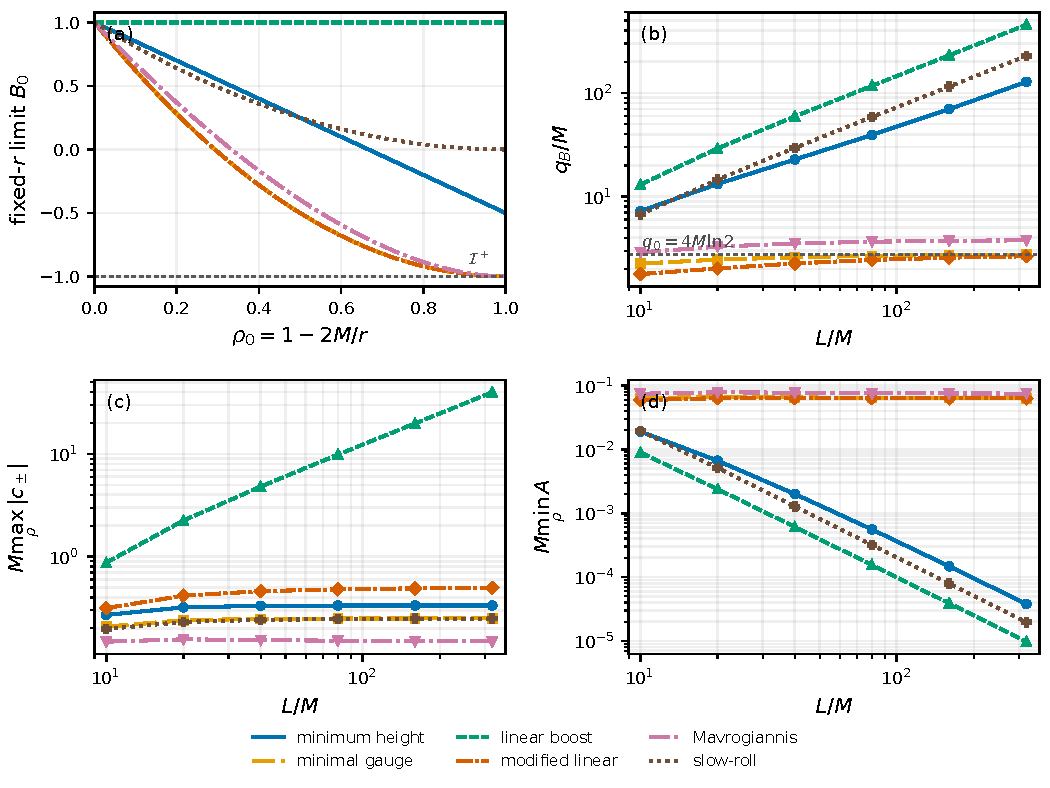
\includegraphics[width=\textwidth]{figs/foliation_flat_limit.pdf}
 \caption{Large-$L$ foliation and coefficient diagnostics.  (a) Fixed-$r$
 boost limits, with the outgoing Schwarzschild hyperboloidal target
 $1+B_0=\mathcal O(M^2/r^2)$ at $\scri^+$.  (b) Offsets from the source to
 the outer horizon,
 $q_B(L;4M)$.  The dotted line is the minimal-gauge Schwarzschild value.
 (c) $M\max_\rho|c_\pm|$ and (d) $M\min_\rho A$ on the compact interval.
 Visual encodings identify each family.  The minimal-gauge and modified-linear
 limits coincide in panel (a).}
 \label{fig:foliation_limit}
\end{figure*}

Panels (c) and (d) connect each asymptotic limit to the numerical
coefficients.  For the linear boost at $L/M=160$,
$M\max|c_\pm|=19.86$ and $M\min A=3.88\times10^{-5}$, with maximum speed
growing linearly in $L/M$.  The minimum of $MA$ falls as $(M/L)^2$ for the
minimum-height and slow-roll families.  Linear slices share this decay in
$A$.  All these values refer to the fixed compactification
\eqref{eq:compactification} and change under a new radial coordinate.  The
minimal and Mavrogiannis gauges keep coefficients of order $M^{-1}$ across
the compact domain.  At $L/M=160$ their
$(M\max|c_\pm|,M\min A)$ pairs are $(0.2498,0.06324)$ and
$(0.1499,0.07495)$.  For the modified-linear family, the desired pointwise
boost limit accompanies a nonuniform outer propagation coefficient:
\begin{equation}
 \lim_{L\to\infty}M A_{\rm fl}(1)=\frac14
 \ne
 \lim_{\rho\to1^-}\lim_{L\to\infty}M A_{\rm fl}(\rho)=\frac18.
\label{eq:modified_linear_layer}
\end{equation}
This mismatch occupies an outer layer that shrinks as $L$ grows.  The
endpoint has $Mc_{+,\rm fl}(1)\to1/2$.  Taking the Schwarzschild limit in the
interior gives $Mc_{+,0}(\scri^+)=1/4$.

We use the minimal gauge because its hyperboloidal limit reproduces the finite
clock in Eq.~\eqref{eq:q_zero} and its coefficients remain bounded across the
compact domain \cite{PanossoMacedo:2023qzp,ZhouPanossoMacedo:2025}.  A
separate closed-form implementation supplies the Schwarzschild reference.
The coefficient diagnostics in
Fig.~\ref{fig:foliation_limit} come from the analytic coefficients,
independently of the waveform evolutions.

\subsection{Direct finite-\texorpdfstring{$L$}{L} recovery}
\label{sec:direct_recovery}

For $\xi=0$, the direct comparison answers the practical scalar-wave
question: how large
must $L/M$ be before a finite cosmological calculation approximates the
chosen Schwarzschild observable?  The answer depends on the observable and
accuracy threshold.  For the cumulative, prompt-dominated pure-$\ell=2$
sequence, agreement including the case-specific numerical margin first
reaches $5\%$ at $L/M=320$ and $2\%$ at $L/M=640$; direct $1\%$ agreement is
not reached through $L/M=640$.  These thresholds do not apply to the
localized-source response.

Across $L/M=20$ through $640$, the boundary waveforms retain the prompt-pulse
and ringdown morphology of the Schwarzschild reference
(Fig.~\ref{fig:flat_sequence}).  In the large-$L$ regime, the dominant
residual amplitude falls by about a factor of two with each doubling of $L$,
while its prompt-interval shape changes little.  This behavior motivates the
expansion in Eq.~\eqref{eq:regulator_expansion}.

\begin{figure*}[t]
 \centering
 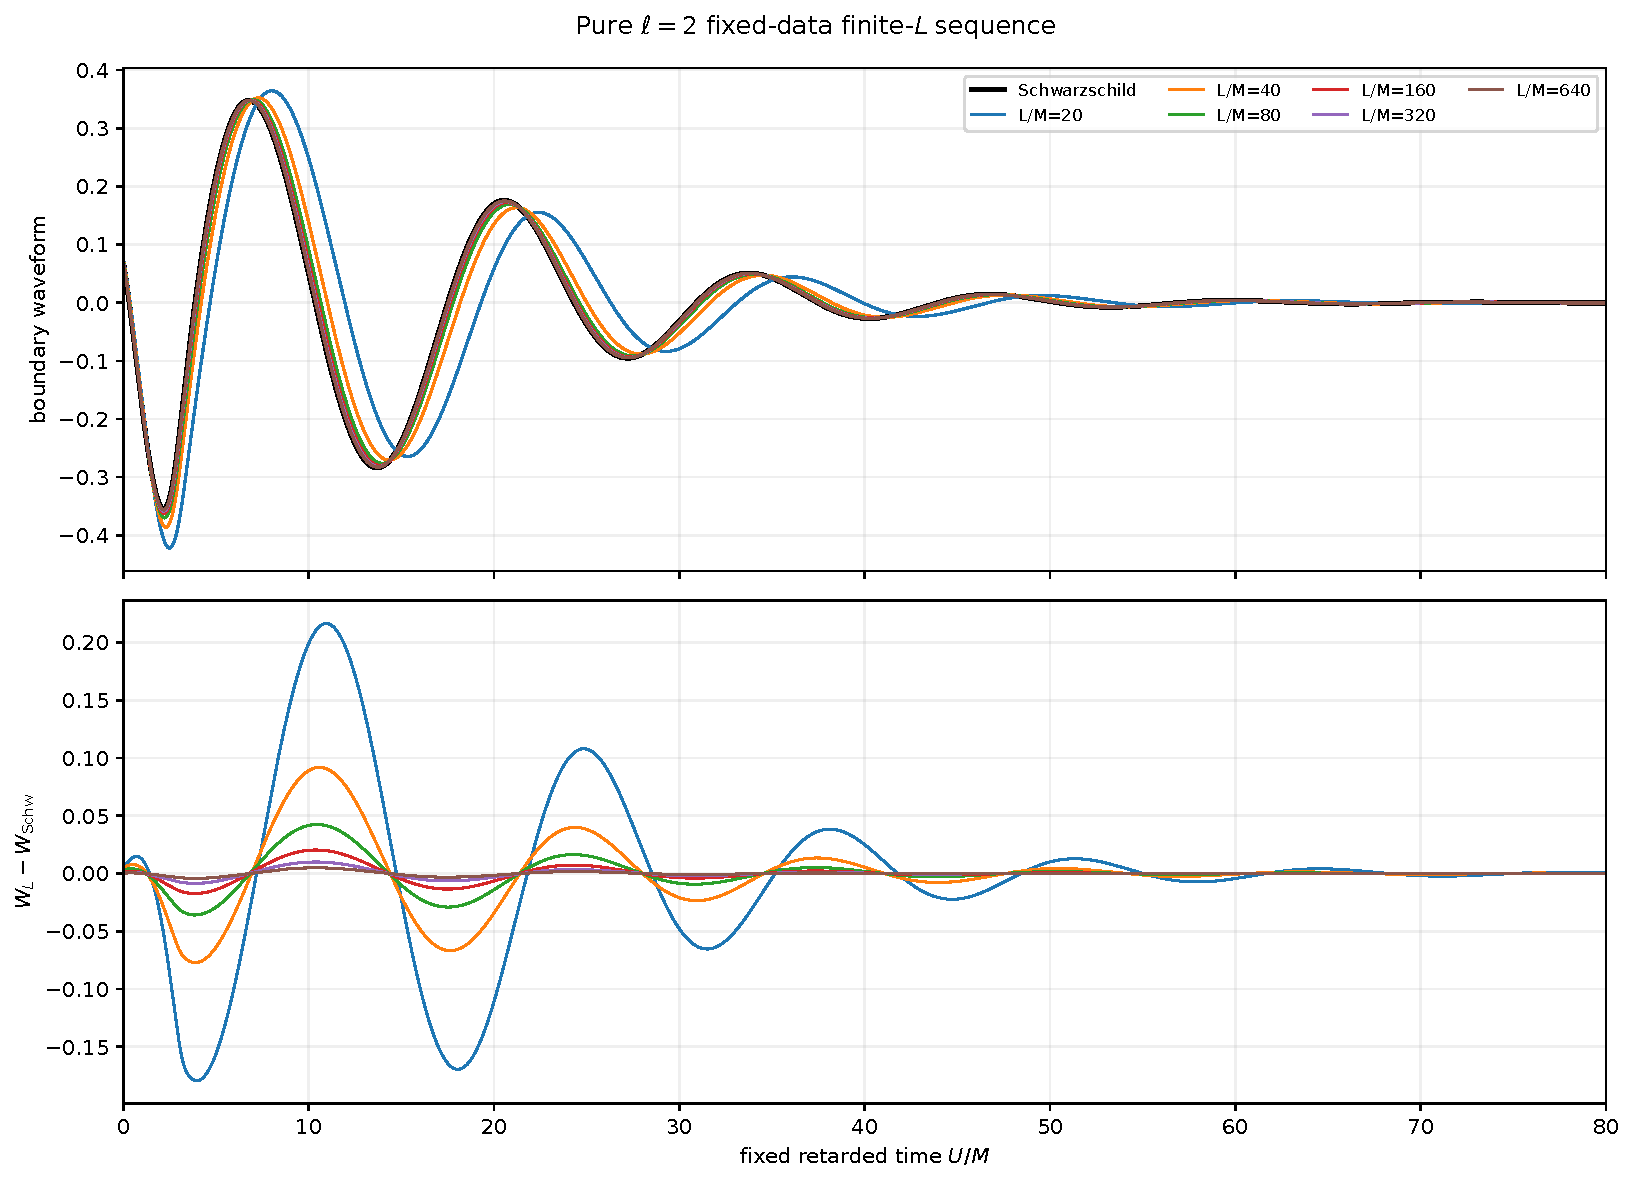
\includegraphics[width=\textwidth]{figs/flat_waveform_sequence.pdf}
 \caption{Minimally coupled ($\xi=0$), fixed-data, pure-$\ell=2$ sequence at
 the outer boundary.  Upper
 panel: waveforms for $L/M=20$ to $640$ against the separately evolved
 Schwarzschild reference.  Lower panel: the residual $W_L-W_{\rm Schw}$ on
 the same retarded time $U=\tau-q_L$, with no relative time translation
 fitted.  The residual amplitude falls with $L$ while its prompt-interval
 morphology changes only weakly.}
 \label{fig:flat_sequence}
\end{figure*}

At fixed $L$, the three cumulative $E_2$ values differ only in the fourth
digit even though the window length increases fourfold
(Table~\ref{tab:flat_windows}), confirming prompt dominance.  Their numerical
scales remain well below the finite-$L$ differences, so the $5\%$ and $2\%$
crossings are resolved properties of the sequence.  On the two disjoint late
intervals, however, the differences approach or cross their numerical scales
(Fig.~\ref{fig:flat_windows}) and support only convergence diagnostics.

\begin{table*}[t]
 \caption{Direct finite-$L$ scalar-wave errors for the minimally coupled,
 fixed-data, pure-$\ell=2$ sequence.  $E_\infty$ is normalized by the largest Schwarzschild amplitude
 in the same interval.  The refinement column is the directly observed
 medium-to-fine paired-residual change in
 Eq.~\eqref{eq:paired_refinement_change}.  These thresholds apply to
 the pure $\ell=2$ family only and not to the localized source.}
\label{tab:flat_windows}
\begin{ruledtabular}
\begin{tabular}{rlrrrl}
$L/M$ & interval & $E_2$ (\%) & $E_\infty$ (\%) & observed refinement (\%) & status\\
\colrule
320 & $0\leq U/M\leq40$ & 2.7161 & 2.8160 & 0.0275 & quantitative\\
320 & $0\leq U/M\leq80$ & 2.7154 & 2.8160 & 0.0643 & quantitative\\
320 & $0\leq U/M\leq160$ & 2.7154 & 2.8160 & 0.1478 & quantitative\\
320 & $40\leq U/M\leq80$ & 2.4145 & 2.0113 & 1.2126 & diagnostic\\
320 & $80\leq U/M\leq160$ & 5.5766 & 1.8859 & 145.1606 & diagnostic\\
640 & $0\leq U/M\leq40$ & 1.3406 & 1.3937 & 0.0114 & quantitative\\
640 & $0\leq U/M\leq80$ & 1.3402 & 1.3937 & 0.0239 & quantitative\\
640 & $0\leq U/M\leq160$ & 1.3402 & 1.3937 & 0.0465 & quantitative\\
640 & $40\leq U/M\leq80$ & 1.1547 & 0.9708 & 0.4380 & diagnostic\\
640 & $80\leq U/M\leq160$ & 7.0146 & 2.0280 & 43.4837 & diagnostic\\
\end{tabular}
\end{ruledtabular}
\end{table*}

\begin{figure*}[t]
 \centering
 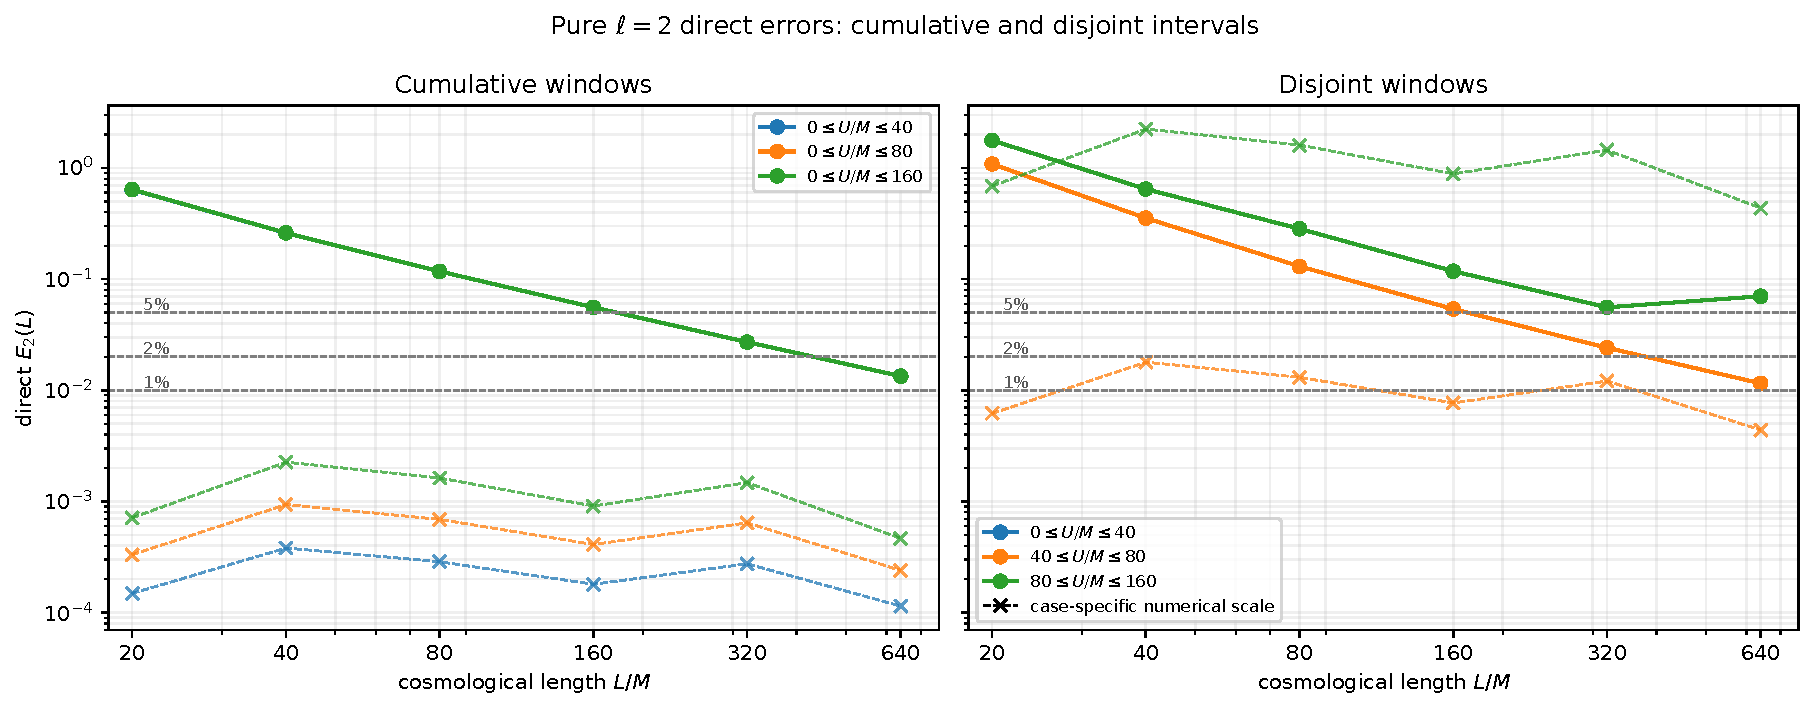
\includegraphics[width=\textwidth]{figs/flat_window_errors.pdf}
 \caption{Direct error $E_2(L)$ for the minimally coupled, fixed-data,
 pure-$\ell=2$ sequence on
 the cumulative intervals (left) and the disjoint intervals (right).  Solid
 curves with filled markers are the differences; dashed curves with crosses
 are the case-specific numerical scales from the same refinement ladder.
 The cumulative curves are prompt dominated and lie well above their
 numerical scale.  On the disjoint intervals the differences approach or
 cross their numerical scales, so those points are diagnostic.}
 \label{fig:flat_windows}
\end{figure*}

\subsection{Nested recovery of the Schwarzschild waveform}
\label{sec:extrapolated_recovery}

For the minimally coupled sequence, the largest pairwise fine-grid residual
across the cumulative windows between
$W_\infty^{(80)}$, $W_\infty^{(160)}$, and the separately evolved
Schwarzschild waveform is $0.0313\%$.  Refinement sets the supported accuracy:
the largest medium-to-fine change of a derived extrapolant is $0.409\%$, and
the largest propagated Richardson estimate is $0.119\%$.  These scales
support a conservative $1\%$ recovery of the tested Schwarzschild waveform.

The extrapolants use the overlapping triples $(80,160,320)$ and
$(160,320,640)$ in units of $L/M$, sharing the $160$ and $320$ calculations.
Their difference tests sensitivity to omitted higher-order terms in
Eq.~\eqref{eq:regulator_expansion}, but does not constitute an independent
replication.  On the cumulative windows, each extrapolant residual is about
$50$ to $125$ times smaller than the direct residual of its largest-$L$
member (Fig.~\ref{fig:nested}).

\begin{figure*}[t]
 \centering
 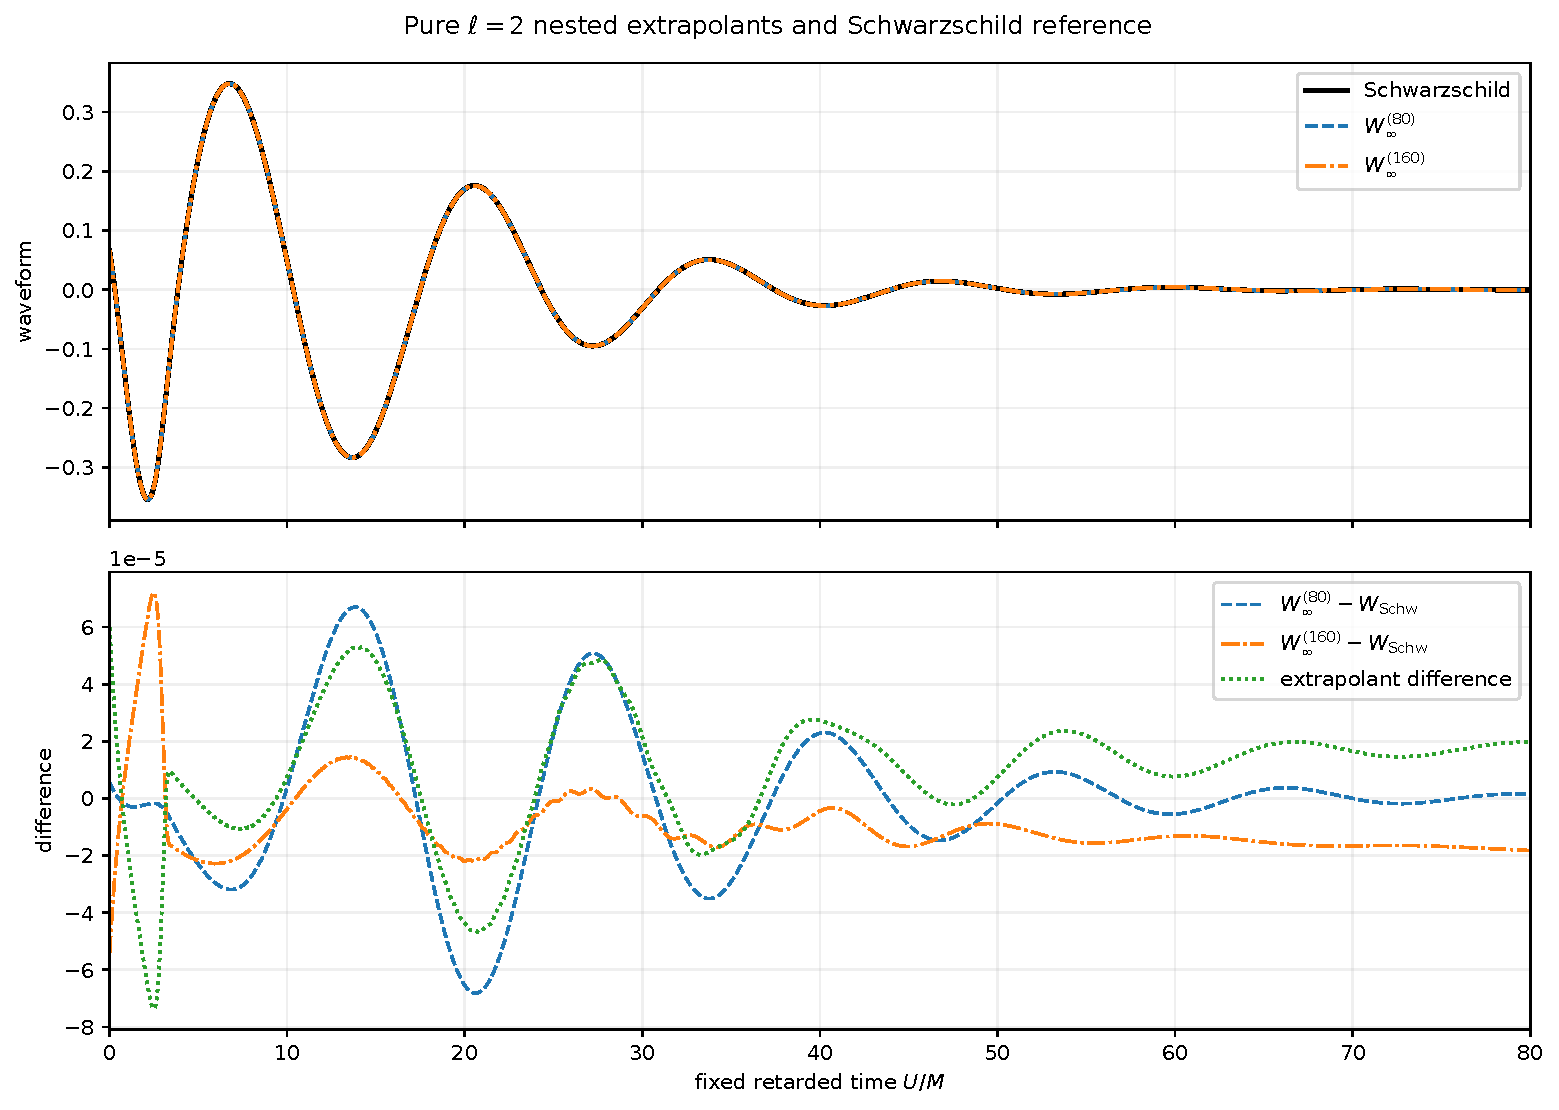
\includegraphics[width=\textwidth]{figs/nested_extrapolants.pdf}
 \caption{Nested extrapolants for the minimally coupled, fixed-data,
 pure-$\ell=2$ sequence.
 Upper panel: $W_\infty^{(80)}$ and $W_\infty^{(160)}$ against the
 separately evolved Schwarzschild waveform.  Lower panel: the two
 residuals and the difference between the overlapping extrapolants, which is
 a correlated diagnostic of omitted higher-order terms.  The plotted range
 ends at $U/M=80$; Table~\ref{tab:extrapolants} also quantifies the
 prompt-dominated cumulative norm through $U/M=160$.}
 \label{fig:nested}
\end{figure*}

Table~\ref{tab:extrapolants} separates the fine-grid residual, paired
medium-to-fine change in Eq.~\eqref{eq:paired_refinement_change}, and
Richardson estimate.  Because refinement exceeds the residual, it sets the
conservative $1\%$ bound.  Appendix~\ref{app:convergence} gives the disjoint
intervals, for which refinement dominates.

\begin{table*}[t]
 \caption{Minimally coupled nested extrapolants on the cumulative intervals,
 each of which
 begins at $U=0$ and ends at $U_{\max}$.  Fine-grid residual, observed
 medium-to-fine paired-residual change, and propagated Richardson estimate are
 distinct quantities and are not combined.}
\label{tab:extrapolants}
\begin{ruledtabular}
\begin{tabular}{lrrrr}
comparison & $U_{\max}/M$ & fine grid & refinement & Richardson\\
 & & (\%) & (\%) & (\%)\\
\colrule
$W_\infty^{(80)}-W_{\rm Schw}$ & 40 & 0.0217 & 0.0469 & 0.0271\\
$W_\infty^{(80)}-W_{\rm Schw}$ & 80 & 0.0222 & 0.1124 & 0.0428\\
$W_\infty^{(80)}-W_{\rm Schw}$ & 160 & 0.0222 & 0.2666 & 0.0777\\
$W_\infty^{(160)}-W_{\rm Schw}$ & 40 & 0.0109 & 0.0190 & 0.0091\\
$W_\infty^{(160)}-W_{\rm Schw}$ & 80 & 0.0142 & 0.0523 & 0.0195\\
$W_\infty^{(160)}-W_{\rm Schw}$ & 160 & 0.0265 & 0.1430 & 0.0413\\
$W_\infty^{(80)}-W_\infty^{(160)}$ & 40 & 0.0186 & 0.0657 & 0.0362\\
$W_\infty^{(80)}-W_\infty^{(160)}$ & 80 & 0.0211 & 0.1643 & 0.0623\\
$W_\infty^{(80)}-W_\infty^{(160)}$ & 160 & 0.0313 & 0.4092 & 0.1189\\
\end{tabular}
\end{ruledtabular}
\end{table*}

\subsection{Localized multimode response}
\label{sec:localized_results}

For $\xi=0$, on the common simulated interval
$0\lesssim U/M\leq57.2$, the localized-source
family extends the benchmark beyond a single spherical harmonic.  In the
sphere-integrated norm \eqref{eq:parseval_norm}, the direct differences are
$E_{2,S^2}(320)=5.267\%$ and $E_{2,S^2}(640)=2.626\%$.  The extrapolants differ
by $0.0517\%$, and each agrees with the separately evolved Schwarzschild
response within the conservative $1\%$ bound.  The interval ends before the
complete late-time signal.  Parseval orthogonality turns the sphere integral
of $|u|^2$ into a sum over modal coefficients and avoids privileging an
observer's location within the caustic pattern.  Figure~\ref{fig:localized}
shows the $\gamma=\pi$ waveform only to illustrate the modal result.

\begin{figure*}[t]
 \centering
 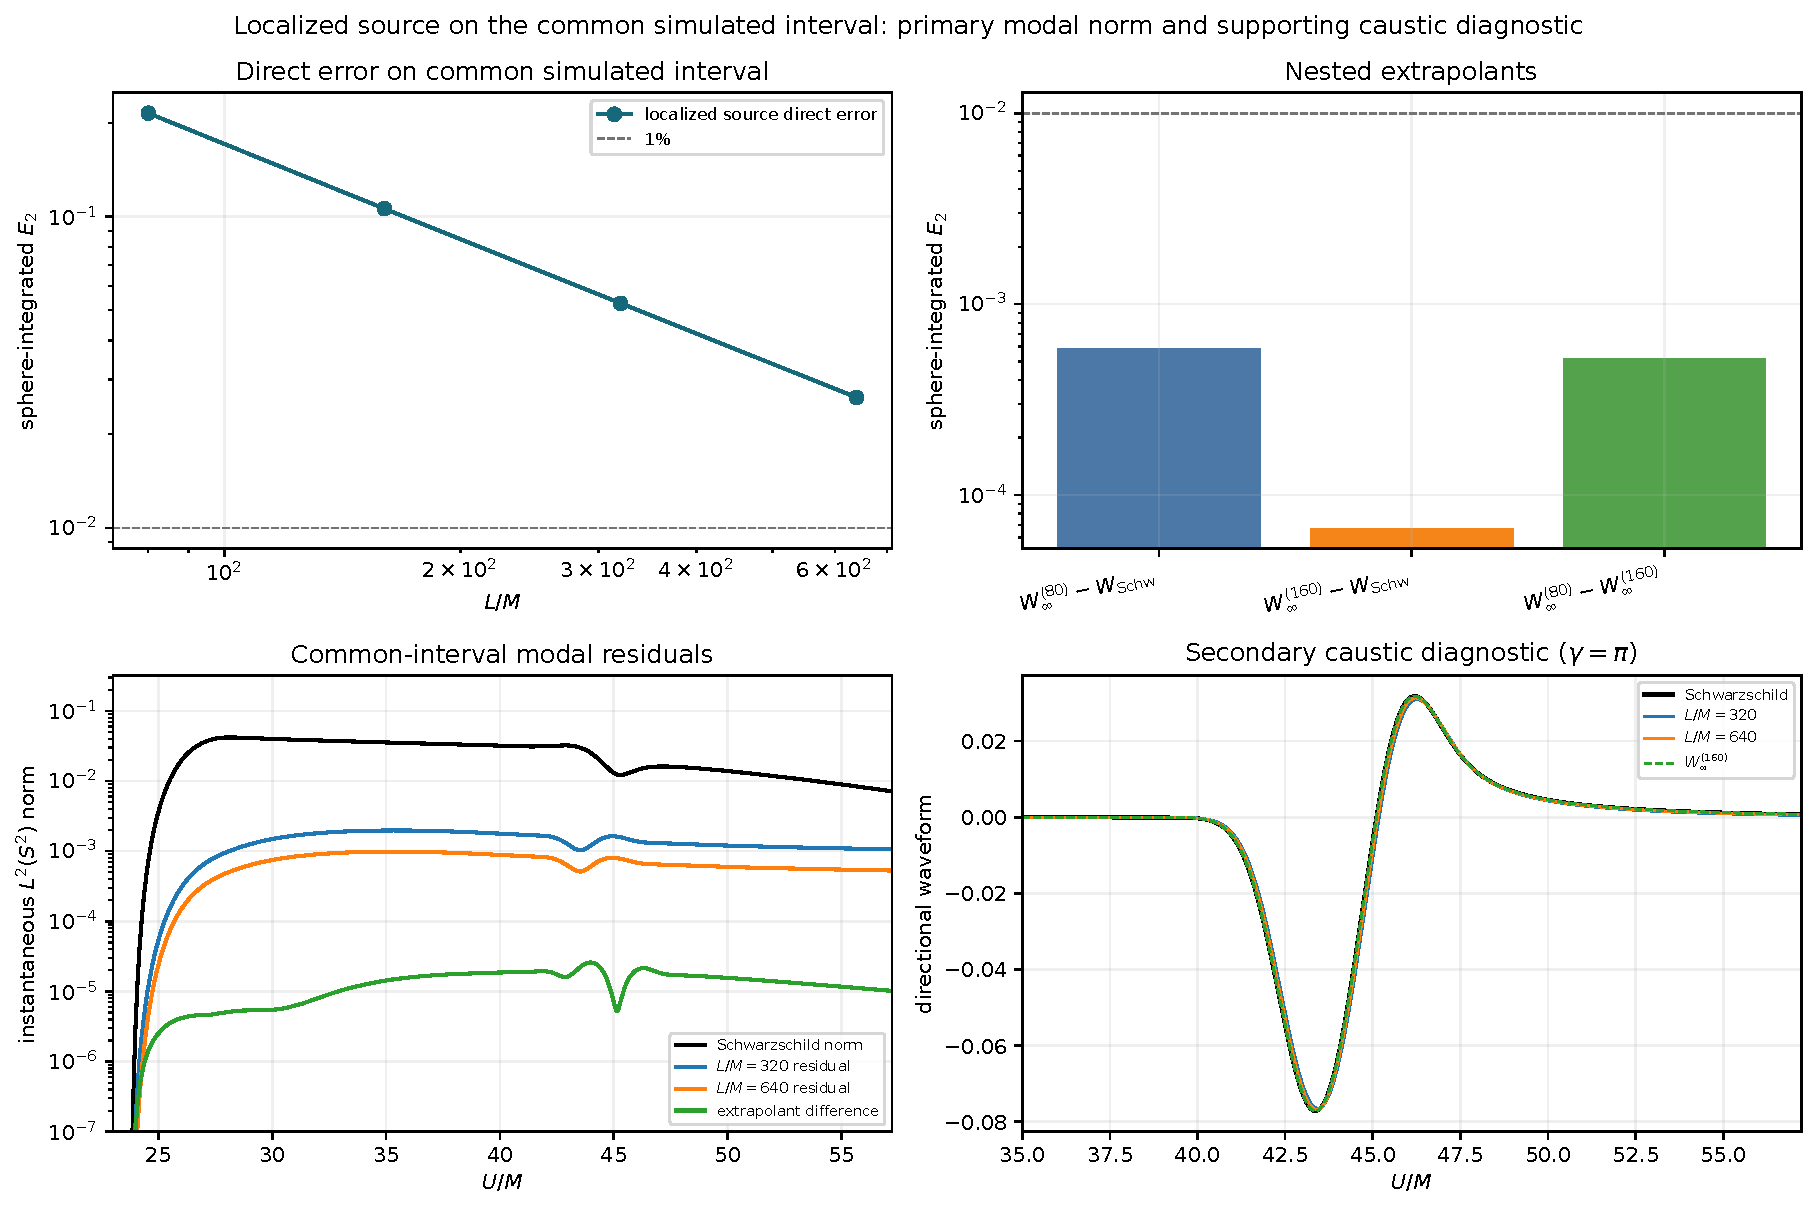
\includegraphics[width=\textwidth]{figs/localized_source_regulator.pdf}
 \caption{Minimally coupled localized source on the common simulated
 interval.  Top left:
 direct sphere-integrated error against $L/M$.  Top right: the three nested
 extrapolant comparisons.  Bottom left: instantaneous $L^2(S^2)$ norms of
 the Schwarzschild response and of the residuals.  Bottom right: the
 caustic direction $\gamma=\pi$, illustrating the reconstructed multimode
 waveform.}
 \label{fig:localized}
\end{figure*}

The medium-to-fine changes in Table~\ref{tab:localized} are at the
$10^{-4}\%$ level, more than a factor of $60$ below the smallest difference; they
establish subdominant refinement, not digit-level accuracy.  The source
parameters in Eqs.~\eqref{eq:source_product}--\eqref{eq:source_angular} are
identical in SdS and Schwarzschild, so emitter width belongs to the physical
problem rather than the error estimate.

\subsection{Supporting Schwarzschild--de Sitter physics}
\label{sec:sds_physics}

The minimally coupled localized response contains caustic echoes that probe
the global SdS
geometry.  We study the shift $D_1$ in the direct-to-first-echo spacing.  Its
scaling is compatible with a local correction of order $(M/L)^2$ at fixed
areal radius and a larger outer response approaching order $M/L$.  The
combined deterministic timing sensitivities exceed the specified tolerance
in all four target-bearing cases, so the fits test these powers but do not
determine precise coefficients.

At a given extraction radius, let $U_{\rm dir}$ denote the arrival of the
direct pulse reconstructed at $\gamma=0$ and let $U_{\rm echo}$ denote the
first caustic echo reconstructed at $\gamma=\pi$.  The primary arrival
estimator is the matched-template lag against the corresponding
Schwarzschild pulse.  We define
\begin{equation}
 D_1(r;L)=
 \left(U_{\rm echo}-U_{\rm dir}\right)_{\mathrm{SdS},L}
 -\left(U_{\rm echo}-U_{\rm dir}\right)_{\mathrm{Schw}},
 \label{eq:d1_definition}
\end{equation}
so any background-independent clock offset cancels.  We include a measurement
in the scaling fit only if all four matched-template lag optimizations avoid
their $\pm4M$ bounds and $|D_1|$ is at least three times its combined
fixed-source deterministic sensitivity.  This threshold excludes both local
$L/M=640$ measurements; Fig.~\ref{fig:d1} retains them as open markers.  The
$1M$ null-geodesic residual threshold applies only to the $L/M=12$
phase pairs in Appendix~\ref{app:convergence} and does not affect the $D_1$
fit.

The near-zone and outer geometries suggest $\mathcal O((M/L)^2)$ and
$\mathcal O(M/L)$ responses, respectively; the data follow these trends
within their deterministic sensitivities (Fig.~\ref{fig:d1}).  We fit
\begin{align}
 \frac{D_{1,\mathrm{local}}}{M}
 &=a_2\left(\frac{M}{L}\right)^2
 +a_4\left(\frac{M}{L}\right)^4,\notag\\
 \frac{D_{1,\mathrm{outer}}}{M}
 &=b_1\frac{M}{L}+b_2\left(\frac{M}{L}\right)^2.
 \label{eq:d1_scaling_models}
\end{align}
We use inverse squared deterministic sensitivities as numerical weights, not
inverse statistical variances.  Accordingly, the curves test the expected
powers only; fitted coefficients and scaled residual sums have no precision
or chi-squared interpretation.  The local fits use $L/M=80$, $160$, and
$320$, while the outer fit also includes $L/M=640$.

A second finite-$\Lambda$ effect in the $\xi=0$ data limits how long a
finite-$L$ calculation can follow Schwarzschild.  At $r=8M$, the $\ell=1$
waveform leaves Schwarzschild
decay at $U=115.9M$ for $L/M=80$ and $133.5M$ for $L/M=160$.  Their near
constancy in units of $M$ points to a black-hole scale.  Cosmological decay
begins at $\kappa_cU=2.83$ and $2.94$; its near constancy in cosmological units
points to $\kappa_c^{-1}$.  The two scales therefore separate as $L$
increases.  The finite-$L$ waveforms depart before a Schwarzschild Price-law
regime is established: the independent reference does not settle within
$5\%$ of its $\ell=1$ power law until $U=220.3M$ at the same radius.  Thus the
finite-$L$ sequence consists of a Schwarzschild-like transient, departure,
and cosmological decay---not a power-law plateau followed by a cosmological
tail.
Appendix~\ref{app:latetime} gives the rate-estimator sweep and radius
dependence.  The separate matched large-$L$ outer-boundary test is reported in
Sec.~\ref{sec:matched-tail-result}; it uses both curvature couplings because
their late SdS targets differ.

%%%%%%%%%%%%%%%%%%%%%%%%%%%%%%%%%%%%%%%%%%%%%%%%%%%%%%%%%%%%%%%%%%%%%%%%%%%%%%%
\clearpage
\begin{center}
\begin{minipage}{\columnwidth}
 \captionof{table}{Minimally coupled localized-source comparison in the
 sphere-integrated modal norm on
 the common simulated interval $0\lesssim U/M\leq57.2$.  The interval
 ends at the last output time shared by all simulations and is not a complete
 late-time signal.}
\label{tab:localized}
\begin{ruledtabular}
\begin{tabular}{lrr}
comparison & $E_{2,S^2}$ (\%) & refinement (\%)\\
\colrule
$W_{320}-W_{\rm Schw}$ & 5.267 & $<0.001$\\
$W_{640}-W_{\rm Schw}$ & 2.626 & $<0.001$\\
$W_\infty^{(80)}-W_{\rm Schw}$ & 0.0584 & $<0.001$\\
$W_\infty^{(160)}-W_{\rm Schw}$ & 0.00672 & $<0.001$\\
$W_\infty^{(80)}-W_\infty^{(160)}$ & 0.0517 & $<0.001$\\
\end{tabular}
\end{ruledtabular}
\end{minipage}
\end{center}
\section{Exterior-supported artificial cosmology}
\label{sec:exterior-supported}
%%%%%%%%%%%%%%%%%%%%%%%%%%%%%%%%%%%%%%%%%%%%%%%%%%%%%%%%%%%%%%%%%%%%%%%%%%%%%%%

The uniform construction modifies the metric throughout the static patch.
Recovering the specified Schwarzschild problem therefore requires large
$L/M$, even when the observable is dominated by the strong-field region.
Misner's cosmological horizon can be retained while the near-zone
modification is removed.  We propose an alternative that keeps the same
exterior value
\begin{equation}
 \Lambda=\frac{3}{L^2}
 \label{eq:exterior_lambda}
\end{equation}
but makes the associated cosmological tensor vanish in a domain containing
the event horizon, initial data, source, photon sphere, and other local
structures.  The main numerical conjecture is that, at fixed exterior
$\Lambda$, this
exterior-supported geometry yields a closer approximation to the same
Schwarzschild waveform than uniform SdS.  If so, it would improve the usable
finite-$L$ representative of the flat limit, or equivalently reach a fixed
waveform tolerance with smaller $L/M$.  The construction is analytically
explicit, and Sec.~\ref{sec:exterior-tests} reports the scalar-wave
comparison.
The construction must also satisfy the global foliation criterion established in
Sec.~\ref{sec:bridges}: regularity at the cosmological horizon alone does not
make the flat limit computable; the bridge, compactification, and waveform
clock must approach the same Schwarzschild problem.

The comparison isolates the effect of relocating the cosmological term.  In
uniform SdS, $-r^2/L^2$ changes the metric even at the photon sphere, and the
scalar potential also depends on $\xi$ through
Eq.~\eqref{eq:uniform_coupled_potential}.  In the exterior-supported family,
the metric, bridge boost, Ricci scalar, and areal-radius potential are exactly
Schwarzschild throughout the initial-data and strong-field region for both
couplings.  Any remaining waveform difference comes from propagation through
the outer layer, the cosmological boundary, and their common clock
construction.  Conformal coupling additionally samples the layer curvature
through $R/6$.  The Schwarzschild, uniform-SdS, and exterior-supported
evolutions therefore separate strong-field bias from outer-propagation bias at
the same $L$.  The matched tail calculation tests the sensitivity of the
outer-propagation result to the two values of $\xi$.
Exact interior shielding follows here from the static spherical ansatz.  In a
generic nonlinear $3+1$ problem, an exterior regulator source enters the
constraint equations and need not leave the near zone exactly unchanged.

\subsection{Conserved cosmological tensor and exact metric}

A coordinate-dependent substitution $\Lambda\mapsto\lambda(r)$ in the
vacuum equations is inconsistent.  Indeed,
\begin{equation}
 G_{ab}+\lambda(r)g_{ab}=0
 \label{eq:variable_lambda_inconsistent}
\end{equation}
and the contracted Bianchi identity would give
\begin{equation}
 0=\nabla^aG_{ab}=-\nabla_b\lambda,
 \label{eq:variable_lambda_bianchi}
\end{equation}
forcing $\lambda$ to be constant.  A consistent spherical construction uses
instead a conserved second-rank tensor,
\begin{equation}
 G^a{}_b+\mathcal{\Lambda}^a{}_b=0,
 \qquad \nabla_a\mathcal{\Lambda}^a{}_b=0,
 \label{eq:cosmological_tensor_equations}
\end{equation}
which becomes $\mathcal{\Lambda}^a{}_b=\Lambda\delta^a{}_b$ wherever the
cosmological term is constant.  Dymnikova introduced the corresponding
radially boost-invariant anisotropic-vacuum structure and its mass-function
interpretation \cite{Dymnikova:2000algebraic,Dymnikova:2002mass}.  Those
works supply the algebraic framework, not the exterior-supported regulator
proposed here.  Our orientation reverses the usual regular-center profile:
the tensor is zero for $r\leq R_0$ and reaches the positive constant-$\Lambda$
form for $r\geq R_1$.

The numerical family follows the original horizon-scaled prescription through
$L_\star/M=160$ and then places a common floor on the transition and cap
widths in Chebyshev angle.  This leaves the $L/M=80$ and $160$ members
unchanged and prevents either outer region from collapsing onto the endpoint.
Define
\begin{equation}
 D_L=1-\frac{2M}{r_c},
 \qquad
 \rho_\chi(r)=\frac{1-2M/r}{D_L},
 \label{eq:exterior_compactification}
\end{equation}
and, on $2M\leq r\leq r_c$, let
$\vartheta(r)=\arccos[2\rho_\chi(r)-1]$.  The Chebyshev collocation points are
uniformly spaced in $\vartheta$.  With $\beta=9/10$, first define
\begin{equation}
\begin{aligned}
 \widehat R_1(L)&=\beta r_c,\\
 \widehat\rho_{\chi,1}(L)&=
 \frac{1-2M/\widehat R_1}{D_L},\\
 \widehat\vartheta_1(L)&=
 \arccos\!\left(2\widehat\rho_{\chi,1}-1\right).
\end{aligned}
 \label{eq:horizon_scaled_transition}
\end{equation}
The final endpoints are
\begin{equation}
\begin{aligned}
 \frac{L_\star}{M}&=160,\\
 \vartheta_\star&=\widehat\vartheta_1(L_\star)
 =0.07526440137447271,\\
 \vartheta_1(L)&=
 \max\{\widehat\vartheta_1(L),\vartheta_\star\},\\
 \vartheta_0(L)&=2\vartheta_1(L),\\
 \rho_{\chi,i}(L)&=\frac{1+\cos\vartheta_i(L)}{2},\\
 R_i(L)&=\frac{2M}{1-D_L\rho_{\chi,i}(L)}
 \quad(i=0,1).
\end{aligned}
 \label{eq:transition_radii}
\end{equation}
Thus $2M<R_0<R_1<r_c$.  For $L\leq L_\star$, the floor is inactive,
$R_1=\beta r_c$, and the transition and cap have equal angle widths,
$\vartheta_0-\vartheta_1=\vartheta_1$.  For $L>L_\star$, both widths equal
$\vartheta_\star$ and both compact endpoints are fixed:
\begin{align}
 \rho_{\chi,0}^\star&=0.9943459581991452,\notag\\
 \rho_{\chi,1}^\star&=0.9985844858695327,\notag\\
 \Delta\rho_{\rm tr}
 &=\rho_{\chi,1}^\star-\rho_{\chi,0}^\star
 =0.004238527670387571,\notag\\
 \Delta\rho_{\rm cap}
 &=1-\rho_{\chi,1}^\star
 =0.001415514130467255.
 \label{eq:transition_compact_widths}
\end{align}
The standard compact $C^\infty$ step is
\begin{align}
 \eta(x)&=
 \begin{cases}
 0,&x\leq0,\\
 e^{-1/x},&x>0,
 \end{cases}
 &
 S(x)&=\frac{\eta(x)}{\eta(x)+\eta(1-x)},
 \label{eq:smooth_step}
\end{align}
The switch and radial cosmological profile are
\begin{equation}
 \chi_L(r)=
 \begin{cases}
 0,&r\leq R_0,\\[1mm]
 S\!\left(\dfrac{\vartheta_0-\vartheta(r)}
 {\vartheta_0-\vartheta_1}\right),&R_0<r<R_1,\\[3mm]
 1,&r\geq R_1,
 \end{cases}
 \label{eq:exterior_switch}
\end{equation}
and set $\lambda(r)=\Lambda\chi_L(r)$.
Then $\chi_L=0$ for $r\leq R_0$, $\chi_L=1$ for $r\geq R_1$, and every
derivative of $\chi_L$ vanishes at both transition endpoints.  The transition
and exact-SdS cap have equal, nonvanishing widths in $\vartheta$ throughout
the family.  Their compact endpoints approach the fixed values above, and
the corresponding areal limits are
\begin{equation}
\begin{aligned}
 \frac{R_{0,\infty}}{M}
 &=\frac{2}{1-\rho_{\chi,0}^\star}
 =353.729256069105,\\
 \frac{R_{1,\infty}}{M}
 &=\frac{2}{1-\rho_{\chi,1}^\star}
 =1412.914189235122,\\
 \frac{R_0}{r_c}&\longrightarrow0,
 &\frac{R_1}{r_c}&\longrightarrow0.
\end{aligned}
 \label{eq:transition_radii_limit}
\end{equation}
The exact-SdS cap still ends at the cosmological horizon, but its inner edge
does not remain at a fixed fraction of that horizon.  The transition begins
and ends at finite, distant radii in the flat limit, while the metric
correction there vanishes as $L^{-2}$.  The entire strong-field region is
exactly Schwarzschild throughout the production sequence, for which
$R_0>6M$.
The metric that preserves the exterior Kottler mass parameter $M$ is
\begin{equation}
 ds^2=-f_\chi(r)dt^2+\frac{dr^2}{f_\chi(r)}+r^2d\omega^2,
 \label{eq:exterior_metric}
\end{equation}
\begin{equation}
 \boxed{\begin{aligned}
 f_\chi(r)&=1-\frac{2M}{r}-\frac{r^2}{3}\lambda(r)\\
 &=1-\frac{2M}{r}-\frac{r^2}{L^2}\chi_L(r).
 \end{aligned}}
 \label{eq:exterior_f}
\end{equation}
It has the exact regional form
\begin{equation}
 f_\chi(r)=
 \begin{cases}
 1-\dfrac{2M}{r},&r\leq R_0,\\[2mm]
 1-\dfrac{2M}{r}-\dfrac{r^2}{L^2}\chi_L(r),
    &R_0<r<R_1,\\[2mm]
 1-\dfrac{2M}{r}-\dfrac{r^2}{L^2},&r\geq R_1.
 \end{cases}
 \label{eq:exterior_f_regions}
\end{equation}
The construction is defined for $M>0$.  Its strong-field region is exactly
Schwarzschild and its exterior is exactly SdS.  The transition is
not vacuum in the ordinary Einstein equations.  It is an exact solution with
a conserved anisotropic effective source, or equivalently a solution of the
modified system \eqref{eq:cosmological_tensor_equations}.

Write
\begin{equation}
 f_\chi=1-\frac{2m_\chi}{r},
 \qquad
 m_\chi(r)=M+\frac{r^3\lambda(r)}{6}.
 \label{eq:exterior_mass_function}
\end{equation}
For a metric in this form,
\begin{equation}
 G^t{}_t=G^r{}_r=-\frac{2m_\chi'}{r^2},
 \qquad
 G^\theta{}_\theta=G^\varphi{}_\varphi=-\frac{m_\chi''}{r}.
 \label{eq:mass_function_einstein}
\end{equation}
It is useful to define source eigenvalues that do not conflict with the
evolution coefficient $A$ or bridge boost $B$,
\begin{align}
 \Lambda_{\parallel}(r)&=\lambda+\frac{r}{3}\lambda',
 \label{eq:lambda_parallel}\\
 \Lambda_{\perp}(r)&=\lambda+r\lambda'
 +\frac{r^2}{6}\lambda''.
 \label{eq:lambda_perp}
\end{align}
The exact cosmological tensor is then
\begin{equation}
 \boxed{\mathcal{\Lambda}^a{}_b
 =\operatorname{diag}\!\left(
 \Lambda_{\parallel},\Lambda_{\parallel},
 \Lambda_{\perp},\Lambda_{\perp}\right)}.
 \label{eq:exterior_cosmological_tensor}
\end{equation}
Equivalently, their nonzero components read
\begin{equation}
 \boxed{\begin{aligned}
 G^t{}_t=G^r{}_r
 &=-\left(\lambda+\frac{r}{3}\lambda'\right),\\
 G^\theta{}_\theta=G^\varphi{}_\varphi
 &=-\left(\lambda+r\lambda'+\frac{r^2}{6}\lambda''\right).
 \end{aligned}}
 \label{eq:exterior_modified_equations}
\end{equation}
The only nontrivial component of the conservation law reduces to
\begin{equation}
 \nabla_a\mathcal{\Lambda}^a{}_r
 =\Lambda_{\parallel}'
 +\frac{2}{r}\left(\Lambda_{\parallel}-\Lambda_{\perp}\right)=0,
 \label{eq:exterior_conservation_check}
\end{equation}
which follows directly from Eqs.~\eqref{eq:lambda_parallel} and
\eqref{eq:lambda_perp}; the other components vanish by stationarity and
spherical symmetry.  Hence
\begin{equation}
 \mathcal{\Lambda}^a{}_b=0\quad(r\leq R_0),
 \qquad
 \mathcal{\Lambda}^a{}_b=\Lambda\delta^a{}_b\quad(r\geq R_1).
 \label{eq:exterior_tensor_regions}
\end{equation}
The derivative terms in the layer are required by conservation and cannot be
discarded.

Placed on the matter side, this tensor gives
\begin{equation}
 T^a{}_b=-\frac{1}{8\pi}\mathcal{\Lambda}^a{}_b
 =\operatorname{diag}(-\varepsilon,p_r,p_\perp,p_\perp),
 \label{eq:exterior_effective_stress}
\end{equation}
where $\varepsilon$ denotes the effective density, avoiding confusion with
the compact coordinate $\rho$,
\begin{equation}
 \varepsilon=\frac{\Lambda_{\parallel}}{8\pi},
 \qquad p_r=-\varepsilon,
 \qquad p_\perp=-\frac{\Lambda_{\perp}}{8\pi}.
 \label{eq:exterior_pressures}
\end{equation}
The radial null energy condition is saturated, whereas the tangential one is
\begin{equation}
 \varepsilon+p_r=0,
 \qquad
 \varepsilon+p_\perp=-\frac{r}{16\pi}\Lambda_{\parallel}'.
 \label{eq:exterior_nec}
\end{equation}
Since
\begin{equation}
 \int_{R_0}^{R_1}\Lambda_{\parallel}'\,dr
 =\Lambda_{\parallel}(R_1)-\Lambda_{\parallel}(R_0)=\Lambda>0,
 \label{eq:exterior_nec_integral}
\end{equation}
$\Lambda_{\parallel}'>0$ somewhere, and the tangential null energy condition
is violated there.  The layer is an artificial regulator medium, not ordinary
matter.  This fact does not by itself preclude numerical use, but it is
central to stability and to any covariant nonlinear completion.

The curvature scalar is
\begin{equation}
 R_\chi=4\lambda+\frac{8}{3}r\lambda'
 +\frac{1}{3}r^2\lambda'',
 \label{eq:exterior_ricci_scalar}
\end{equation}
and equals zero in the interior and $4\Lambda$ in the exterior.  All
curvature quantities are smooth across the layer and throughout the
black-hole exterior; the usual Schwarzschild singularity at $r=0$ remains
when $M>0$.  A useful unexpanded diagnostic is
\begin{equation}
 R_{ab}R^{ab}
 =2\left(\Lambda_{\parallel}^2+\Lambda_{\perp}^2\right),
 \label{eq:exterior_ricci_squared}
\end{equation}
and the Kretschmann scalar is
\begin{equation}
 R_{abcd}R^{abcd}=f_\chi''{}^2
 +4\left(\frac{f_\chi'}{r}\right)^2
 +4\left(\frac{1-f_\chi}{r^2}\right)^2.
 \label{eq:exterior_kretschmann}
\end{equation}
The Misner--Sharp mass accumulated across the transition is
\begin{align}
 \Delta m_{\rm tr}=m_\chi(R_1)-m_\chi(R_0)
 &=\frac{\Lambda R_1^3}{6}=\frac{R_1^3}{2L^2},
 \label{eq:transition_mass_dimensional}\\
 \boxed{\frac{\Delta m_{\rm tr}}{M}}
 &=\frac12\frac{(R_1/M)^3}{(L/M)^2}.
 \label{eq:transition_mass}
\end{align}
Because $R_1$ tends to a finite areal radius in the final family,
\begin{equation}
 \frac{\Delta m_{\rm tr}}{M}
 \sim\frac12\left(\frac{R_{1,\infty}}{M}\right)^3
 \left(\frac{M}{L}\right)^2
 \longrightarrow0.
 \label{eq:transition_mass_fixed_angle_family}
\end{equation}
The tested sequence is still preasymptotic: at $L/M=640$ this quantity is
$104.2917$, which is not perturbatively small.  Its large value is compatible
with small local curvature because the source is diffuse and distant, but the
fixed-background scalar experiment does not show that such a layer can act as
a weak source in nonlinear Einstein evolution.  We record it as a global
diagnostic.  Numerical suitability for the scalar benchmark is tested through
the curvature, scalar potential, compactified coefficients, returned
radiation, and cost.

For a generic layer of areal width $\Delta=R_1-R_0$,
\begin{equation}
 \lambda'=\mathcal O\!\left(\frac{\Lambda}{\Delta}\right),
 \qquad
 \lambda''=\mathcal O\!\left(\frac{\Lambda}{\Delta^2}\right).
 \label{eq:transition_derivative_scales}
\end{equation}
A narrow areal layer can generate large curvature and a sharp scattering
feature.  Here both endpoints have finite limits and
$\Delta\to1059.184933166017M$.  The limiting profile therefore has
$\chi_L'=\mathcal O(M^{-1})$ and
$\chi_L''=\mathcal O(M^{-2})$.  At fixed $M$, the strict large-$L$ scalings
of $\lambda=3\chi_L/L^2$ are
\begin{equation}
 \lambda'=\mathcal O(L^{-2}M^{-1}),
 \qquad
 \lambda''=\mathcal O(L^{-2}M^{-2}).
 \label{eq:transition_width_floored_derivative_scales}
\end{equation}
The combinations entering the source eigenvalues and Ricci curvature are
$\mathcal O(L^{-2})$.  The construction therefore replaces
distributed strong-field bias by a smooth, low-curvature modification in a
distant region.  The lapse change near the cosmological horizon remains order
unity, while the transition retains a fixed spectral width.

The bounds $0\leq\chi_L\leq1$ imply
\begin{equation}
 f_{\rm SdS}(r)\leq f_\chi(r)\leq f_{\rm Schw}(r).
 \label{eq:exterior_metric_bounds}
\end{equation}
For subextremal SdS, $f_{\rm SdS}>0$ between its black-hole and
cosmological roots.  On $(2M,R_0]$, the new metric is exactly Schwarzschild
and $f_\chi>0$.  For $r\geq R_0>6M$, one is outside the SdS black-hole root,
so $f_\chi\geq f_{\rm SdS}>0$ up to $r_c$.  Hence the intended choice
$R_0>6M$ and $R_1<r_c$ guarantees
\begin{equation}
 f_\chi(r)>0\qquad(2M<r<r_c)
 \label{eq:exterior_no_extra_horizon}
\end{equation}
and excludes a transition-region horizon.  Root finding remains a useful
implementation check, especially for profiles that overshoot or transitions
that begin closer to the black hole.  Layer sharpness alone cannot create a
root in the bounded profile above, although it can create large curvature and
potential structure.  The exact near-horizon geometry gives
\begin{equation}
 r_{b,\chi}=2M,
 \qquad \kappa_{b,\chi}=\frac{1}{4M},
 \label{eq:exterior_black_hole_horizon}
\end{equation}
while $r_c$ is the usual exterior root
\begin{equation}
 1-\frac{2M}{r_c}-\frac{r_c^2}{L^2}=0.
 \label{eq:exterior_cosmological_horizon}
\end{equation}
If $R_0>6M$, the inner photon sphere, innermost stable circular orbit, and
black-hole surface gravity take their exact Schwarzschild values,
\begin{equation}
 r_{\rm ph}=3M,
 \qquad r_{\rm ISCO}=6M,
 \qquad \kappa_{b,\chi}=\frac{1}{4M}.
 \label{eq:exterior_local_structures}
\end{equation}
The transition can nevertheless create additional light rings or circular
orbit structure.  This local agreement is necessary but not sufficient for
QNM agreement.  It
suggests that the photon-sphere branch and leading eikonal behavior may be
close \cite{CardosoEtAl:2009geodesic}, but finite-$\ell$ QNMs solve a global
boundary-value problem involving the full exterior potential and both
horizons.

\subsection{Flat-limit-adapted bridge and compactification}

For the $M>0$ black-hole case, the production bridge adapted to
Eq.~\eqref{eq:exterior_f} is
\begin{equation}
 \boxed{B_\chi(r)=-1+\frac{8M^2}{r^2}
 -\frac{8M^2}{r_c^2}\chi_L(r)}.
 \label{eq:exterior_bridge}
\end{equation}
It obeys
\begin{equation}
 B_\chi(2M)=+1,
 \qquad B_\chi(r_c)=-1.
 \label{eq:exterior_bridge_endpoints}
\end{equation}
Because $0\leq\chi_L\leq1$, one has $-1<B_\chi<1$ for
$2M<r<r_c$; since $\chi_L=1$ outside the layer, $B_\chi<-1$ for
$r>r_c$.  The height follows from
\begin{equation}
 h_\chi'(r)=\frac{B_\chi(r)}{f_\chi(r)}.
 \label{eq:exterior_height}
\end{equation}
This choice is convenient, but neither unique nor numerically optimized.
Its horizon crossings are regular; for example,
\begin{align}
 \lim_{r\to2M^+}\frac{1-B_\chi^2}{f_\chi}&=8,\notag\\
 \lim_{r\to r_c^-}\frac{1-B_\chi^2}{f_\chi}
 &=\frac{16M^2}{r_c(r_c-3M)}>0.
 \label{eq:exterior_bridge_regular_limits}
\end{align}
Above $L_\star$, both compact endpoints are fixed.  The limiting switch can
therefore remain nonzero at a fixed radius above $R_{0,\infty}$ and equals one
above $R_{1,\infty}$.  Nevertheless, for fixed $r$ the
last term in Eq.~\eqref{eq:exterior_bridge} is
$\mathcal O(M^2/L^2)$ because $r_c=\mathcal O(L)$.  Therefore
\begin{equation}
 B_\chi(r)=-1+\frac{8M^2}{r^2}
 \qquad(L\to\infty),
 \label{eq:exterior_bridge_flat_limit}
\end{equation}
which is the minimal-gauge Schwarzschild boost in
Eq.~\eqref{eq:schwarz_coefficients}.  Similarly,
$r^2\chi_L/L^2\to0$ in Eq.~\eqref{eq:exterior_f}.  The metric and bridge thus
recover Schwarzschild on every fixed physical-radius interval even though
$\chi_L$ itself can have a nonzero limiting profile there.

The compactification in Eq.~\eqref{eq:exterior_compactification} places $2M$
at $\rho_\chi=0$ and $r_c$ at $\rho_\chi=1$ and tends to
$1-2M/r$ as $L\to\infty$.  Its conformal factor may be chosen as
\begin{equation}
 \Omega_{\chi,L}=\frac{2M}{r},
 \qquad \Omega_{\chi,L}(1)=\frac{2M}{r_c}>0,
 \label{eq:exterior_conformal_factor}
\end{equation}
with $\Omega_{\chi,L}(1)\to0$ in the Schwarzschild limit.  Smaller $L$ increases
this nonzero endpoint value and may strengthen the regulator effect.  Whether
it improves the regularity or conditioning of conformal Einstein evolution
remains an open numerical question.

The coefficients used in Eqs.~\eqref{eq:evolve_u}--\eqref{eq:evolve_pi} are
obtained without numerical differentiation of the compactification:
\begin{align}
 G_\chi&=\frac{2M}{D_Lr^2},&
 A_\chi&=\frac{f_\chi G_\chi}{1-B_\chi^2},\notag\\
 P^\chi_{\ell,\xi}&=\frac{D_L}{2M}
 \left[\ell(\ell+1)+rf_\chi'+\xi r^2R_\chi\right].
 \label{eq:exterior_scalar_coefficients}
\end{align}
Their removable horizon limits are assigned analytically, as in
Eq.~\eqref{eq:A_endpoint}.
In the exact-SdS cap, the horizon equation gives
$D_L=r_c^2/L^2=1-2M/r_c$.  The outer endpoint values are therefore
\begin{align}
 A_\chi(1)&=\frac{r_c-3M}{8M(r_c-2M)},&
 c_{+,\chi}(1)&=2A_\chi(1),\notag\\
 P^\chi_{\ell,\xi}(1)&=\frac{D_L}{2M}
 \left[\ell(\ell+1)-2+\frac{6M}{r_c}\right.\notag\\
 &\left.\hspace{7em}+12\xi D_L\right].
 \label{eq:exterior_outer_endpoint_coefficients}
\end{align}
Hence
\begin{align}
 A_\chi(1)&\longrightarrow\frac{1}{8M},&
 c_{+,\chi}(1)&\longrightarrow\frac{1}{4M},\notag\\
 P^\chi_{\ell,0}(1)&\longrightarrow
 \frac{\ell(\ell+1)-2}{2M},&
 P^\chi_{\ell,1/6}(1)&\longrightarrow
 \frac{\ell(\ell+1)}{2M}.
 \label{eq:exterior_outer_endpoint_flat_limit}
\end{align}
The principal coefficients thus recover their Schwarzschild endpoint values.
Conformal coupling also recovers $P_{\rm Schw}(1)$, whereas minimal coupling
retains the same lower-order endpoint offset as uniform SdS.  Because every
member ends in an exact-SdS cap, moving the transition outward cannot remove
this nonuniformity.  It supplies an analytic mechanism for the tail
sensitivity tested below.  The finite-$L$ family converges geometrically on
compact physical-radius sets and in its endpoint principal part and clock; it
does not converge uniformly in every lower-order compactified coefficient.

With the same normalization $r_0=4M$, define
\begin{equation}
 q_\chi=\int_{r_0}^{r_c}\frac{1+B_\chi}{f_\chi}\,dr,
 \qquad U=\tau-q_\chi.
 \label{eq:exterior_clock}
\end{equation}
The endpoint is regular because
\begin{equation}
 \lim_{r\to r_c}\frac{1+B_\chi}{f_\chi}
 =\frac{B_\chi'(r_c)}{f_\chi'(r_c)}
 =\frac{8M^2}{r_c(r_c-3M)}.
 \label{eq:exterior_clock_endpoint}
\end{equation}
The clock limit contains fixed-radius and horizon-scale pieces.  Choose a
fixed $R>R_{1,\infty}$.  For sufficiently large $L$, the complete transition
lies below $R$ and $[R,r_c]$ is exactly SdS.  On $[r_0,R]$, the integrand
converges to its Schwarzschild minimal-gauge value with
$\mathcal O(L^{-2})$ corrections.  In the exact cap it can be evaluated in
the cancellation-free form
\begin{equation}
 \frac{1+B_\chi}{f_\chi}
 =\frac{8M^2(r_c+r)}{r^2r_c^2
 \left[(r_c+r)/L^2-2M/(rr_c)\right]}.
 \label{eq:exterior_clock_cap}
\end{equation}
Comparison with the integrable Schwarzschild tail then gives
\begin{equation}
 q_\chi=q_0-\frac{8M^2}{r_c}
 +o\!\left(\frac{M^2}{r_c}\right)
 \longrightarrow q_0=4M\ln\frac{r_0}{r_0-2M}.
 \label{eq:exterior_clock_flat_limit}
\end{equation}
Thus the fixed-angle-width exterior-supported family shares the common
Schwarzschild clock used above.  The production audit records $q_\chi$ at
every $L$ and compares it with the asymptotic formula in
Eq.~\eqref{eq:exterior_clock_flat_limit}.

\subsection{Minimally coupled production comparison}
\label{sec:exterior-tests}

The completed $\xi=0$ calculation tests a fixed-background hypothesis:
moving the
cosmological modification out of the strong-field region should reduce the
scalar waveform error at the same exterior $\Lambda$.  Exact Schwarzschild
geometry inside $R_0$ does not prove this statement because waves still cross
the transition and satisfy an outgoing condition at $r_c$.  We therefore use
the same physical datum, waveform clock, Schwarzschild reference, and
uniform-SdS controls as in Sec.~\ref{sec:direct_recovery}.

The production sequence reported here uses $\xi=0$, the compact
pure-$\ell=2$ datum, and
$L/M=80,160,320,640$.  The $L/M=80$ and $160$ members are algebraically
unchanged by the final floor and their longer validated archives are truncated
to the common analysis interval.  The $L/M=320$ and $640$ members were evolved
afresh to $\tau=100M$.  All runs use RK222, $3/2$ dealiasing, and waveform
output every $0.03M$.  The coarse, medium, and fine spatial resolutions are,
in increasing $L/M$ order,
\begin{equation}
\begin{aligned}
 L/M=80:&\quad(384,512,768),\\
 L/M=160:&\quad(768,1024,1536),\\
 L/M=320:&\quad(1024,1536,2048),\\
 L/M=640:&\quad(768,1024,1536).
\end{aligned}
 \label{eq:exterior_resolution_ladders}
\end{equation}
The corresponding timesteps are $0.005M$, $0.00375M$, and $0.0025M$ for
every $L$, matching the control ladder.  In these $\xi=0$ archives, the
bounded zeroth-order potential is explicit in the IMEX split and transport
remains implicit.  Because space
and time are refined together, the numerical scale below measures their
coupled refinement.  A fixed-resolution timestep check would separate the two
errors but is not used to reduce the quoted scale.

The angle floor is active at $L/M=320$ and $640$.  Their audited transition
radii are
\begin{equation}
\begin{array}{c|cc}
 L/M & R_0/M & R_1/M\\ \hline
 320 &168.2329417&260.5413505\\
 640 &228.1477989&440.4330107
\end{array}
 \label{eq:fixed_angle_transition_radii}
\end{equation}
The respective fine grids place $49/49$ and $37/37$ Chebyshev points in the
transition/cap pair.  For $\xi=0$, the $L/M=640$
potential-representation error is $3.47\times10^{-6}$ relative to the
analytic transition minimum.  Every background, spectral, and
evolution-stability guard for this production sequence passes.

For either coupling, the scalar potential is
\begin{equation}
 V_{\ell,\xi}^\chi=f_\chi\left[
 \frac{\ell(\ell+1)}{r^2}+\frac{f_\chi'}{r}+\xi R_\chi\right].
 \label{eq:exterior_scalar_potential}
\end{equation}
Using Eqs.~\eqref{eq:exterior_metric} and
\eqref{eq:exterior_ricci_scalar}, the conformally coupled specialization is
\begin{equation}
 V_{\ell,1/6}^\chi=f_\chi\left[
 \frac{\ell(\ell+1)}{r^2}+\frac{2M}{r^3}
 +\frac{r\lambda'}{9}+\frac{r^2\lambda''}{18}\right].
 \label{eq:exterior_conformal_scalar_potential}
\end{equation}
It equals the Schwarzschild potential inside $R_0$ and the conformally
coupled SdS potential outside $R_1$.  The derivative terms in the transition
show why the $\xi=1/6$ potential needs an independent resolution audit.
The bounds in Eq.~\eqref{eq:exterior_metric_bounds} exclude unintended roots
analytically.  Before an archive is accepted, a dense background audit also
checks $f_\chi>0$ and $|B_\chi|<1$ between the horizons, finite compactified
coefficients, and, for the completed $\xi=0$ sequence, a nonnegative
represented potential.  The conformal audit instead checks that the
curvature-dependent potential is finite and spectrally resolved; it imposes
no sign condition.  A dense-versus-spectral comparison of the appropriate
transition potential checks that the transition's nonvanishing
compact-coordinate width is resolved.  The preflight
also verifies the active endpoint branch and both intended angle widths.  It
enforces prescribed minimum transition and cap point counts separately; the
common angle floor protects both counts above $L_\star$.  The machine-readable
audit records $r_c$, $R_0$, $R_1$, the compact widths and point counts,
$q_\chi$, coefficient extrema, potential resolution,
$\Delta m_{\rm tr}/M$, runtime, and step count.  It also compares the maximum
stored reduction-constraint norms across the refinement ladder; it does not
infer an interval-resolved constraint history from endpoint snapshots.
A loose acceptance guard also rejects nonfinite evolution or order-of-magnitude
growth in the stored waveforms, snapshots, or reduction constraint.  This is
a blow-up check, not an accuracy estimate; accuracy still comes from the
three-level waveform comparison.

Against the same separately evolved Schwarzschild waveform $W_{\rm Schw}$, define
\begin{equation}
 E_X(L;\mathcal J)
 =\frac{\|W_X-W_{\rm Schw}\|_{\mathcal J}}{\|W_{\rm Schw}\|_{\mathcal J}},
 \qquad X\in\{\mathrm{SdS},\chi\}.
 \label{eq:exterior_waveform_error}
\end{equation}
All comparisons use the raw outer-boundary waveform: no time translation,
amplitude rescaling, time dilation, or transfer correction is fitted.  The
focused post-production comparison defines the operational QNM window as
$15\leq U/M\leq45$.  Equal-duration windows
$10$--$40M$ and $20$--$50M$ test sensitivity to this choice; the overlapping
windows are correlated diagnostics, not independent measurements.  The
prompt-inclusive $0$--$80M$ norm remains a secondary audit.  These $100M$
evolutions do not address the long-time tail or a possible late return from
the layer.

For each family, successive-grid changes are computed from its residual
$W_X-W_{\rm Schw}$ and normalized by $\|W_{\rm Schw}\|_{\mathcal J}$.  If they decrease,
$\eta_X$ is the larger of the medium--fine change and the estimated remaining
fine-grid scale.  For a nonmonotone ladder, $\eta_X$ is instead the larger of
the two successive changes, and no Richardson order is assigned.  We call the
observed-grid ordering margin-separated when
$E_\chi+\eta_\chi<E_{\rm SdS}-\eta_{\rm SdS}$.  The common Schwarzschild
reference floor enters absolute accuracy thresholds but is not counted twice
when deciding which family is closer to the same frozen reference.  All four
central-window fine-grid orderings remain separated under the more pessimistic
check that adds this floor to the exterior upper bound and subtracts it from
the uniform lower bound.  This criterion does not by itself imply continuum
convergence.

Figure~\ref{fig:exterior-qnm-residuals} compares the signed residuals.  Moving
the cosmological term outward reduces the residual norm across each ringdown
window, without a fitted time shift or amplitude rescaling.

\begin{figure*}[t]
 \centering
 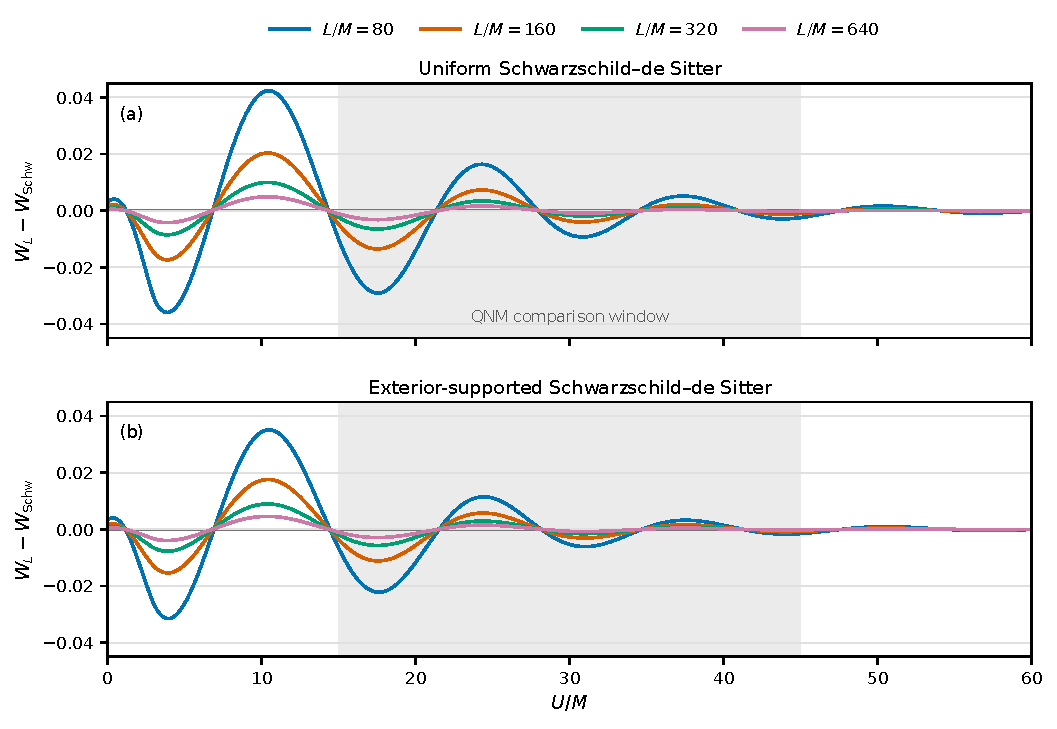
\includegraphics[width=\textwidth]{figs/exterior_qnm_residual_comparison.pdf}
 \caption{Minimally coupled ($\xi=0$) raw fine-grid residuals relative to the
 same Schwarzschild waveform for uniform SdS (top) and the exterior-supported
 family (bottom).  Both
 panels use identical axes and colors.  Shading marks the nominal
 $15\leq U/M\leq45$ operational QNM window.  No fitted time shift or amplitude
 rescaling has been applied; interpolation only places the signals on the
 common Schwarzschild $U$ grid.}
 \label{fig:exterior-qnm-residuals}
\end{figure*}

Table~\ref{tab:exterior-qnm-improvement} quantifies the comparison.  On the
nominal window the error reduction decreases from $25.7\%$ at $L/M=80$ to
$8.6\%$ at $L/M=640$, while all three windows give a positive reduction at
every $L$.  Each nominal improvement clears the adopted family-specific
numerical margins.  The $L/M=640$ exterior ladder is nonmonotone, so its
$\eta_\chi$ is the larger observed level-to-level change.  Its observed-grid
ordering is margin-separated, not continuum-converged.

\begin{table*}[t]
\caption{Minimally coupled ($\xi=0$) raw QNM-window agreement with
 Schwarzschild.  Errors and numerical scales refer to
 $15\leq U/M\leq45$ and are percentages; $\eta$ is a
 conservative coupled refinement scale, not a statistical uncertainty.  The
 $L/M=640$ exterior value is the larger observed level-to-level change and
 has no Richardson interpretation.  The
 last column gives the relative-reduction range across the fixed
 $10$--$40M$, $15$--$45M$, and $20$--$50M$ windows.}
\label{tab:exterior-qnm-improvement}
\begin{ruledtabular}
\begin{tabular}{rrrrrrr}
$L/M$ & $100E_{\rm SdS}$ & $100\eta_{\rm SdS}$
& $100E_\chi$ & $100\eta_\chi$
& reduction (\%) & window range (\%)\\
\hline
80  &14.593&0.0756&10.839&0.0178&25.7&20.9--30.2\\
160 & 6.679&0.0472& 5.446&0.00521&18.5&15.6--21.2\\
320 & 3.189&0.0725& 2.780&0.00146&12.8&11.3--14.3\\
640 & 1.558&0.0299& 1.424&0.0176& 8.6& 7.8--9.3\\
\end{tabular}
\end{ruledtabular}
\end{table*}

The prompt-inclusive $0$--$80M$ audit gives smaller central reductions of
$18.0\%$, $14.1\%$, $10.5\%$, and $7.35\%$ as $L/M$ increases.  In the
$40$--$80M$ disjoint window the improvement is unresolved at $L/M=320$ and
$640$, so the sequence supports no late-time claim.

This comparison is deliberately narrower than the uniform-SdS study.  It
tests the background change with one clean fixed-mode datum; it does not
repeat the localized-source calculation.  The improved raw ringing waveform
is not a separate determination of quasinormal frequencies or damping rates.
The exact Schwarzschild photon sphere protects the local eikonal structure,
but finite-$\ell$ quasinormal frequencies depend on the full potential and
both boundaries.  We therefore make no claim about the global quasinormal
spectrum of the exterior-supported geometry.

\subsection{Matched outer-boundary tail result}
\label{sec:matched-tail-result}

The QNM-window comparison above ends before the broad secondary structure
seen in the long runs develops.  Tails pose a distinct test because they depend on the global
scattering problem.  We therefore evolve matched $\ell=1$, $L/M=640$
waveforms through $U/M=1000$ for Schwarzschild, uniform SdS, and the
exterior-supported geometry.  The Schwarzschild waveform is measured at
$\scri^+$; both finite-$L$ waveforms are measured at $\hc$.  Each finite-$L$
geometry is evolved with $\xi=0$ and $1/6$, while the Schwarzschild reference
is common because $R[g]=0$.

Figure~\ref{fig:matched-tail} shows the signed waveforms, root-mean-square
envelopes, and local power indices.  The Schwarzschild signal settles to
$p_{\rm eff}=3$.  The local decay index for uniform conformal SdS enters the
same band for a substantial intermediate interval.  Neither
exterior-supported signal does so.  Instead,
both exterior cases develop a slowly decaying component followed by broad
secondary lobes.  Unweighted least-squares fits of $\ln A$ against $\ln U$
on the resolved $N=3072$ envelopes give $A\sim U^{-1.086}$
($R^2=0.9926$) for $\xi=0$ on $120\leq U/M\leq250$ and
$A\sim U^{-0.920}$ ($R^2=0.9911$) for $\xi=1/6$ on
$160\leq U/M\leq400$.  These exponents describe the chosen transition
profile over finite intervals; they are not universal tail indices.

\begin{figure*}[!t]
 \centering
 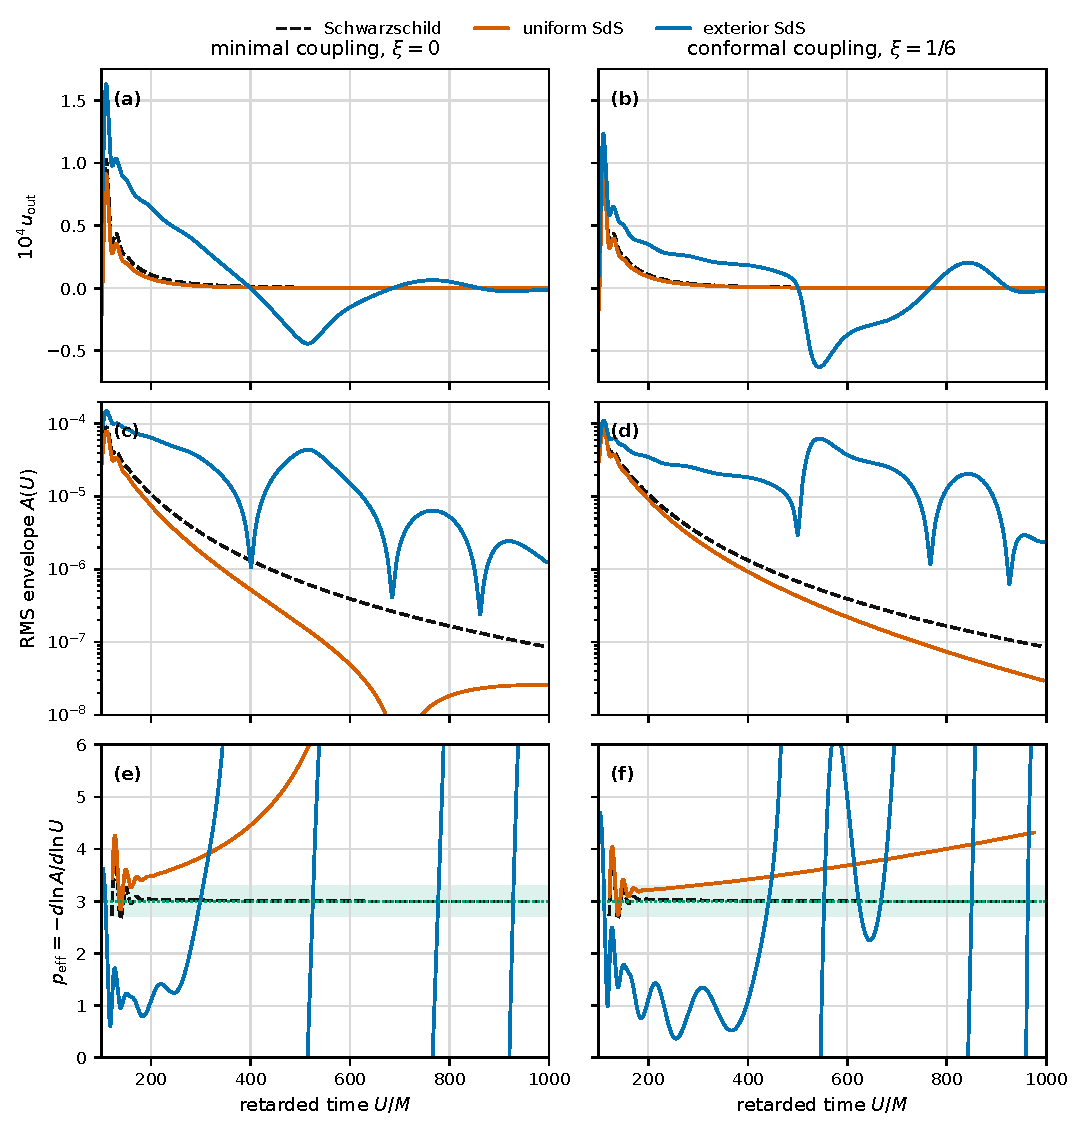
\includegraphics[width=\textwidth]{figs/tail_outer_boundary_comparison.pdf}
 \caption{Matched $\ell=1$, $L/M=640$ outer-boundary tail comparison for
 minimal coupling (left) and conformal coupling (right).  The rows show the
 signed fine-grid waveform, its centered $10M$ root-mean-square envelope, and
 the local power index from a centered $40M$ log--log fit.  Schwarzschild is
 extracted at $\scri^+$; uniform and exterior-supported SdS are extracted at
 $\hc$.  The shaded band marks $p_{\rm eff}=3\pm10\%$.  Power indices are
 drawn only where the envelope exceeds ten times the measured spatial or
 temporal refinement floor, the $N=2048$ and $3072$ indices agree within
 $0.1$, and the full- and half-step $N=2048$ indices agree within $0.1$;
 neighborhoods of signed zero crossings are omitted.  Neither a time
 shift nor an amplitude rescaling is fitted to the waveforms.}
 \label{fig:matched-tail}
\end{figure*}

Table~\ref{tab:matched-tail} applies the acceptance criterion defined in
Appendix~\ref{app:latetime}.  Among the finite-$L$ cases, only uniform
conformal SdS sustains $p_{\rm eff}=3\pm10\%$ for the required $40M$.
All nine combinations of $5M$, $10M$, and $20M$ envelope widths with $30M$,
$40M$, and $60M$ rate-fit widths give the same pass/fail classification.
For the positive uniform-conformal result, the relative waveform changes
over the exact $153.3$--$294.8M$ interval are $7.90\times10^{-5}$ from
$N=1536$ to $2048$ and $7.97\times10^{-6}$ from $N=2048$ to $3072$;
halving the timestep at $N=2048$ changes the waveform by
$3.23\times10^{-8}$.  The $141.5M$ interval is therefore refinement
supported.

\begin{table*}[t]
\caption{Longest refinement-supported candidate intervals within
$p_{\rm eff}=3\pm10\%$ for the matched $\ell=1$, $L/M=640$ calculation.
The primary estimator uses a centered $10M$ root-mean-square envelope and a
centered $40M$ local fit.  Passing requires a duration of at least $40M$.
The upper Schwarzschild endpoint is the last admissible center of the
finite-record estimator, not a physical departure from the Price law.}
\label{tab:matched-tail}
\begin{ruledtabular}
\begin{tabular}{lcccc}
geometry & $\xi$ & candidate interval $U/M$ & duration$/M$ & $40M$ criterion\\
\colrule
Schwarzschild & --- & $140.4$--$975.0$ & $\geq834.7$ & pass\\
uniform SdS & $0$ & $134.5$--$144.1$ & $9.6$ & fail\\
exterior-supported SdS & $0$ & $292.9$--$304.8$ & $11.9$ & fail\\
uniform SdS & $1/6$ & $153.3$--$294.8$ & $141.5$ & pass\\
exterior-supported SdS & $1/6$ & $618.7$--$628.0$ & $9.4$ & fail\\
\end{tabular}
\end{ruledtabular}
\end{table*}

The null result for the exterior family is resolved.  Its three spatial
grids use $N=1536$, $2048$, and $3072$, all with
$\Delta\tau/M=0.0025$; an $N=2048$ run with half that timestep isolates the
temporal sensitivity.  On the successive windows $300$--$500M$,
$500$--$750M$, and $750$--$950M$, the $N=2048$--$3072$ relative waveform
changes are respectively $2.41\times10^{-6}$, $3.80\times10^{-6}$, and
$2.97\times10^{-5}$ for $\xi=0$, and $4.28\times10^{-5}$,
$3.15\times10^{-5}$, and $1.34\times10^{-4}$ for $\xi=1/6$.  The preceding
spatial differences are larger by factors of about $10$--$11$ and
$7.4$--$7.6$, respectively, so the changes decrease rapidly under
refinement.  Halving the timestep
changes the same signals by only $3$--$4\times10^{-8}$, and the largest stored
reduction-constraint norm in either exterior ladder is
$1.09\times10^{-8}$.  The slow components and secondary lobes therefore do
not converge away.  The independent endpoint-factored evolution in
Appendix~\ref{app:tail-formulation-check} gives the same failed Price-interval
classification and the same slow exterior component, so this conclusion does
not depend on the shared-flux reduction.

With a centered semilog fit window $\Delta(\kappa_cU)=0.25$, neither uniform
waveform develops a refinement-supported interval within $10\%$ of its
expected asymptotic rate, $\gamma/\kappa_c=1$ for $\xi=0$ or $2$ for
$\xi=1/6$.  No target is imposed on the exterior geometry, and no exterior
asymptotic rate is quoted.  For $L/M=640$, the record reaches only
$\kappa_cU=1.558$, so we report neither an asymptotic rate nor a cosmological
entry time.  The combined result is narrower
than a general failure of artificial cosmology: exterior support improves the
prompt ringing waveform, but the tested tail remains sensitive to the complete
outer construction---the transition, exact-SdS cap, and cosmological
boundary.  The data do not isolate these contributions.

\subsection{Scope and acceptance criteria}

The completed $\xi=0$ fixed-background calculation supports the proposal in
a limited sense:
at fixed exterior $\Lambda$, exterior support gives an observed-grid reduction
of the short ringing-waveform error that is separated by conservative
level-to-level margins.  The background audits exclude extra
horizons and an unresolved transition potential, and every QNM-window
evolution remains stable through $100M$.  The dedicated tail ladders remain
stable through $U/M=1000$ and resolve the later exterior-supported signal;
they do not establish long-time computational efficiency.  The transition
mass is not perturbatively small on the tested sequence and limits its
nonlinear interpretation; it does not invalidate the fixed-background scalar
comparison.  These conclusions concern only scalar waves on a fixed spherical
background.  Exact shielding is therefore a property of this static spherical
background, not a result about initial data satisfying the nonlinear Einstein
constraints.

The nonlinear Einstein problem supplies the broader motivation but is not
part of this benchmark.  The spherical construction uses invariant areal
radius.  A generic three-dimensional implementation could instead attach the
support to an outer gauge coordinate or to a regulator field, which is
compatible with standard $3+1$ infrastructure but adds structure whose
conservation and dynamics must be specified.
Moreover, gravitational perturbations must satisfy
\begin{equation}
 \delta\!\left(\nabla_a\mathcal{\Lambda}^a{}_b\right)=0.
 \label{eq:perturbed_conservation}
\end{equation}
In general, one cannot hold $\mathcal{\Lambda}^a{}_b$ fixed while perturbing
the metric; its perturbations and dynamics must be specified.  Background
feasibility, scalar test-field feasibility, and gravitational feasibility are
therefore distinct claims.  The scalar model cannot establish preservation
of gravitational QNMs or the viability of a nonlinear regulator.  A later
Einstein test would require a dynamical regulator field, a covariant
anisotropic medium, or another conserved compensating source, together with
constraint, conservation, hyperbolicity, regularity, stability, accuracy, and
cost checks.

%%%%%%%%%%%%%%%%%%%%%%%%%%%%%%%%%%%%%%%%%%%%%%%%%%%%%%%%%%%%%%%%%%%%%%%%%%%%%%%
\section{Conclusions}
\label{sec:conclusions}

For the completed minimally coupled ($\xi=0$) scalar benchmark, artificial
cosmology is a coherent limiting construction, not merely a choice of positive
cosmological constant.  The metric, foliation, compactification,
initial-data map, and waveform clock must all select the
same asymptotically flat problem.  Local regularity at the cosmological
horizon does not ensure this limit: the continuation of the slices beyond
that horizon determines which Schwarzschild end is recovered.  The minimal
gauge used here has the required global end, a finite limiting
clock, and bounded, nondegenerate compactified scalar-wave coefficients.

The $\xi=0$ calculation tests background selection, data matching, clock
alignment, waveform comparison, and extrapolation on fixed black-hole backgrounds.  Its
validation strategy is to choose a globally compatible finite-$L$ family,
hold the physical comparison fixed, measure direct errors, and test nested
extrapolation against a separately evolved asymptotically flat reference.  For
the tested observables, direct SdS waveforms approach their Schwarzschild
counterparts as $L/M$ grows, but no single finite-$L$ run reproduces
Schwarzschild uniformly across all observables and times.  The two nested
extrapolants support agreement at a conservative $1\%$ level for the
cumulative, prompt-dominated fixed-mode test and for the localized multimode
response on its common simulated interval.  The unresolved disjoint late-time
windows do not support the same bound.

The minimally coupled localized calculation also supplies a fully
angle-dependent $3+1$
benchmark for scalar propagation on a black-hole background, with the
cosmological horizon as the finite-$L$ outer boundary and $\scri^+$ for the
Schwarzschild reference.  It reconstructs a multimode field from independently
propagated radial responses by using the exact modal decoupling of the
spherical background.  The response also exposes genuine finite-$\Lambda$
physics: caustic timing is consistent with a near-zone correction of order
$(M/L)^2$ and an outer response approaching order $M/L$, although deterministic
extraction sensitivities preclude precision coefficient claims.

These $\xi=0$ fixed-background results provide a quantitative prerequisite for
Misner's proposal.  They neither evolve the nonlinear Einstein equations nor
test the regularization or conditioning of their formally singular conformal
source terms.  The fact that $\Omega_L$ remains nonzero at finite $L$ is the
proposal's geometric premise, not a numerical regularity result.

In the static spherical background used here, the minimally coupled
exterior-supported construction in Sec.~\ref{sec:exterior-supported} leaves
the strong-field metric exactly Schwarzschild and trades distributed
finite-$L$ bias for a distant conserved anisotropic layer.  Fixing nonzero
Chebyshev-angle widths for both the
transition and exact-SdS cap makes the sequence computable through
$L/M=640$.  With the same scalar data, clock, norms, Schwarzschild reference,
and uniform-SdS controls, exterior support reduces the raw QNM-window error at
every tested $L$.  The nominal reduction decreases from $25.7\%$ at $L/M=80$
to $8.6\%$ at $L/M=640$.  The ladders are monotone through $L/M=320$; at
$L/M=640$ the nonmonotone observed-grid ordering remains separated under
conservative level-to-level margins but is not continuum-converged.  This is a
short-time waveform result, not a determination of the global QNM spectrum.
This QNM-window reduction has not been established
for $\xi=1/6$ and should not be inferred from the matched tail calculation.

The long-time test gives the complementary limitation.  Uniform conformal
SdS resolves a $141.5M$ intermediate interval consistent with the
Schwarzschild $U^{-3}$ Price law, but uniform minimal SdS and both
exterior-supported couplings fail the declared $40M$ persistence test.  The
exterior waveforms instead develop convergent slow components and broad
secondary lobes.  Moving the cosmological modification outward therefore
improves the prompt ringing sector but does not protect a tail that probes the
global asymptotic structure.  Neither uniform case resolves its expected
asymptotic cosmological rate by $U/M=1000$; no target is assigned to the
exterior family.  The calculation therefore supports no fitted crossover
time.  This
coupling-dependent result is a physical boundary on the regulator test, not a
numerical failure.

A nonlinear implementation also requires a covariant, conserved completion;
prescribing a coordinate-dependent scalar $\Lambda(r)$ is inconsistent with
the Bianchi identity.  Beyond the fixed-background benchmark,
the motivating nonlinear Einstein
evolution at finite $L$ must be followed by the same controlled large-$L$
comparison.  Such a calculation
must assess how finite $L$ treats the formally singular source terms, monitor
constraint behavior and gauge conditioning, and compare waveform accuracy and
computational cost with direct-$\scri^+$ formulations.  Full-GR hyperboloidal
evolution at $\scri^+$ has advanced substantially in spherical symmetry, but
a robust generic three-dimensional metric free-evolution scheme with
$\scri^+$ fixed as the outer grid boundary and compatible with
binary-black-hole infrastructure remains open.  Artificial cosmology may
help to overcome that obstacle; establishing whether it does requires the
nonlinear Einstein code that lies beyond this scalar study.

%%%%%%%%%%%%%%%%%%%%%%%%%%%%%%%%%%%%%%%%%%%%%%%%%%%%%%%%%%%%%%%%%%%%%%%%%%%%%%%
\appendix

\section{Numerical verification and deterministic sensitivities}
\label{app:convergence}

Every numerical value in this appendix belongs to a $\xi=0$ evolution.  The
uniform fixed-mode and localized-source production families use the
three-level ladders of Sec.~\ref{sec:scalar}, and each waveform comparison is
formed at all three levels.  The observed refinement change is the
medium-to-fine norm of the paired residual-waveform difference in
Eq.~\eqref{eq:paired_refinement_change}; it is not the scalar difference of
two reported $E_2$ values.  The Richardson estimate uses the order observed
from the coarse, medium, and fine sequence together with the resolution ratio
to estimate the remaining fine-level scale under that order.  The two answer
different questions and are never added or averaged; where they disagree the
larger enters the direct threshold tests.

The exterior-supported comparison applies the same paired-residual principle
separately to the uniform and exterior families.  Its conservative scale is
defined below Eq.~\eqref{eq:exterior_waveform_error}.  The QNM-window exterior ladders are
monotone for $L/M=80$, $160$, and $320$; the $L/M=640$ ladder is not, so no
Richardson order is assigned there.  The largest stored reduction-constraint
norm over the new $L/M=320$ and $640$ runs is $2.87\times10^{-3}$, and all
background, representation, and stability guards pass.  The family-specific
scales used in the comparison are given explicitly in
Table~\ref{tab:exterior-qnm-improvement}.

For the fixed-mode family the largest cumulative refinement change is
$0.1478\%$ at $L/M=320$ and $0.0465\%$ at $L/M=640$, with Richardson
estimates $0.0138\%$ and $0.0035\%$.  Derived extrapolants inherit the
refinement of all three members, which is why their observed changes reach
$0.409\%$ while their fine-grid residuals stay near $0.03\%$.
Table~\ref{tab:extrapolant_audit} carries the complete extrapolant audit.
On the disjoint intervals refinement dominates: fine-grid residuals of $0.096$
to $0.211\%$ on $40\leq U/M\leq80$ carry refinement changes of $1.02$ to
$3.14\%$, and on $80\leq U/M\leq160$ refinement exceeds the residual
outright, which is the sole reason those rows appear as diagnostics rather
than as late-time accuracy statements.  For the localized source family the
observed refinement changes stay at the $10^{-4}\%$ level on the archived
interval.

The standalone Schwarzschild check compares complete archived fields with a
sphere and time integrated Parseval norm.  Relative to the fine
$(N_r,\Delta\tau/M,\ell_{\max})=(2048,0.0005,50)$ archive, the coarse and
medium ladder differences are $3.44\times10^{-7}$ and
$7.66\times10^{-8}$.  Truncating the fine response itself isolates angular
omission from radial and temporal error; the relative omitted-field norms are
$2.29\times10^{-9}$ at $\ell_{\max}=42$ and $1.26\times10^{-10}$ at
$\ell_{\max}=46$.  The largest stored reduction constraint is
$1.80\times10^{-11}$.  No relative clock shift enters these checks.

\begin{table*}[t]
 \caption{Complete minimally coupled ($\xi=0$) nested-extrapolant audit for
 the fixed-data, pure-$\ell=2$ sequence.  The fine-grid residual, the directly observed medium-to-fine
 paired-residual change, and the propagated Richardson estimate are distinct
 quantities.  A row is diagnostic when refinement is not subdominant.}
\label{tab:extrapolant_audit}
\begin{ruledtabular}
\begin{tabular}{llrrrl}
comparison & interval & fine-grid residual (\%) & observed refinement (\%) & Richardson estimate (\%) & status\\
\colrule
$W_\infty^{(80)}-W_{\rm Schw}$ & $0\leq U/M\leq40$ & 0.0217 & 0.0469 & 0.0271 & $1\%$ test\\
$W_\infty^{(80)}-W_{\rm Schw}$ & $0\leq U/M\leq80$ & 0.0222 & 0.1124 & 0.0428 & $1\%$ test\\
$W_\infty^{(80)}-W_{\rm Schw}$ & $0\leq U/M\leq160$ & 0.0222 & 0.2666 & 0.0777 & $1\%$ test\\
$W_\infty^{(80)}-W_{\rm Schw}$ & $40\leq U/M\leq80$ & 0.0957 & 2.1322 & 0.7704 & diagnostic\\
$W_\infty^{(80)}-W_{\rm Schw}$ & $80\leq U/M\leq160$ & 0.8518 & 263.6959 & 73.7109 & diagnostic\\
$W_\infty^{(160)}-W_{\rm Schw}$ & $0\leq U/M\leq40$ & 0.0109 & 0.0190 & 0.0091 & $1\%$ test\\
$W_\infty^{(160)}-W_{\rm Schw}$ & $0\leq U/M\leq80$ & 0.0142 & 0.0523 & 0.0195 & $1\%$ test\\
$W_\infty^{(160)}-W_{\rm Schw}$ & $0\leq U/M\leq160$ & 0.0265 & 0.1430 & 0.0413 & $1\%$ test\\
$W_\infty^{(160)}-W_{\rm Schw}$ & $40\leq U/M\leq80$ & 0.1882 & 1.0164 & 0.3665 & diagnostic\\
$W_\infty^{(160)}-W_{\rm Schw}$ & $80\leq U/M\leq160$ & 24.3986 & 145.1404 & 39.9353 & diagnostic\\
$W_\infty^{(80)}-W_\infty^{(160)}$ & $0\leq U/M\leq40$ & 0.0186 & 0.0657 & 0.0362 & $1\%$ test\\
$W_\infty^{(80)}-W_\infty^{(160)}$ & $0\leq U/M\leq80$ & 0.0211 & 0.1643 & 0.0623 & $1\%$ test\\
$W_\infty^{(80)}-W_\infty^{(160)}$ & $0\leq U/M\leq160$ & 0.0313 & 0.4092 & 0.1189 & $1\%$ test\\
$W_\infty^{(80)}-W_\infty^{(160)}$ & $40\leq U/M\leq80$ & 0.2105 & 3.1441 & 1.1369 & diagnostic\\
$W_\infty^{(80)}-W_\infty^{(160)}$ & $80\leq U/M\leq160$ & 24.6156 & 408.7846 & 113.6462 & diagnostic\\
\end{tabular}
\end{ruledtabular}
\end{table*}

A minimally coupled sourced configuration has also been run through both
implementations at
$L/M=80$ on Schwarzschild and SdS as a separate validation data set rather
than as part of either production sequence.  Across
those archives the largest sphere-integrated relative difference between the
two implementations is
$5.58\times10^{-4}$ and the largest individual arrival difference is
$4.14\times10^{-4}M$.  That comparison used the analytic envelope arrival on
both sides, whereas the $D_1$ analysis of Sec.~\ref{sec:sds_physics} uses
the matched template lag as its primary estimator.  The two are therefore
reported as separate checks: the cross implementation numbers validate the
sourced waveform and timing pipeline, and are not combined with the
matched template values as measurements of one observable.
Both validation runs use $\ell_{\max}=42$, $\Delta\tau=0.002M$, output every
$0.002M$, and end at $72M$.  The finite difference run uses $N_r=768$ and
classical RK4.  The Dedalus run uses 512 Chebyshev T modes, a $3/2$ dealias
factor, RK443, and stagewise source evaluation.

Table~\ref{tab:timing} separates the deterministic timing sensitivities.
The PDE column comes from the paired refinement ladder; the estimator column
from the difference between matched template and analytic envelope arrivals;
the window column from four displacements and rescalings of the fixed
extraction windows by $0.5M$; and the cadence column from analysis grids at
$0.0005M$, $0.001M$, and $0.002M$.  The combined column is their linear sum,
which is a conservative deterministic bound and not a standard deviation, a
confidence interval, or a fit weight with a $\chi^2$ interpretation.  The
specified combined analysis targets fail at every entry, although the PDE
contributions alone would meet them.  Dependence on the source width is a
physical property of the chosen emitter, is available only from the
separate earlier fixed-background width study, and is excluded from this fixed
source target by construction.

\begin{table*}[t]
 \caption{Minimally coupled ($\xi=0$) deterministic timing sensitivities in
 units of $M$.  The combined
 column is a conservative linear sum and not a statistical error.  None of
 the four target-bearing entries meets its specified analysis criterion,
 while every PDE contribution alone would.  The
 associated $D_1$ scaling is therefore used only as consistency evidence.}
\label{tab:timing}
\begin{ruledtabular}
\begin{tabular}{rlrrrrrr}
$L/M$ & observer & PDE & estimator & window & cadence & combined & target\\
\colrule
320 & $r=8M$ & $6.80\times10^{-8}$ & $3.24\times10^{-4}$ & $2.52\times10^{-5}$ & $3.04\times10^{-7}$ & $3.49\times10^{-4}$ & $1.0\times10^{-4}$\\
320 & $r=12M$ & $7.86\times10^{-7}$ & $7.83\times10^{-4}$ & $1.59\times10^{-5}$ & $4.47\times10^{-8}$ & $8.00\times10^{-4}$ & $1.0\times10^{-4}$\\
320 & outer & $3.83\times10^{-9}$ & $4.03\times10^{-3}$ & $2.45\times10^{-4}$ & $2.21\times10^{-6}$ & $4.28\times10^{-3}$ & $5.0\times10^{-4}$\\
640 & outer & $1.04\times10^{-8}$ & $2.11\times10^{-3}$ & $1.27\times10^{-4}$ & $1.56\times10^{-6}$ & $2.24\times10^{-3}$ & $5.0\times10^{-4}$\\
\end{tabular}
\end{ruledtabular}
\end{table*}

Two exclusions are recorded rather than corrected.  Both local $L/M=640$
timings are diagnostic because $|D_1|$ is not large compared with the
combined sensitivity of the same measurement.  All six generic angle phase
pairs at $L/M=12$ are excluded from quantitative phase analysis because at
least one extracted pulse in each pair differs from its null geodesic
arrival by more than the $1M$ tolerance, the largest residual being
$15.666M$.  No phase estimate is reported for those pairs, and their
rejection carries no physical interpretation.

\begin{figure*}[t]
 \centering
 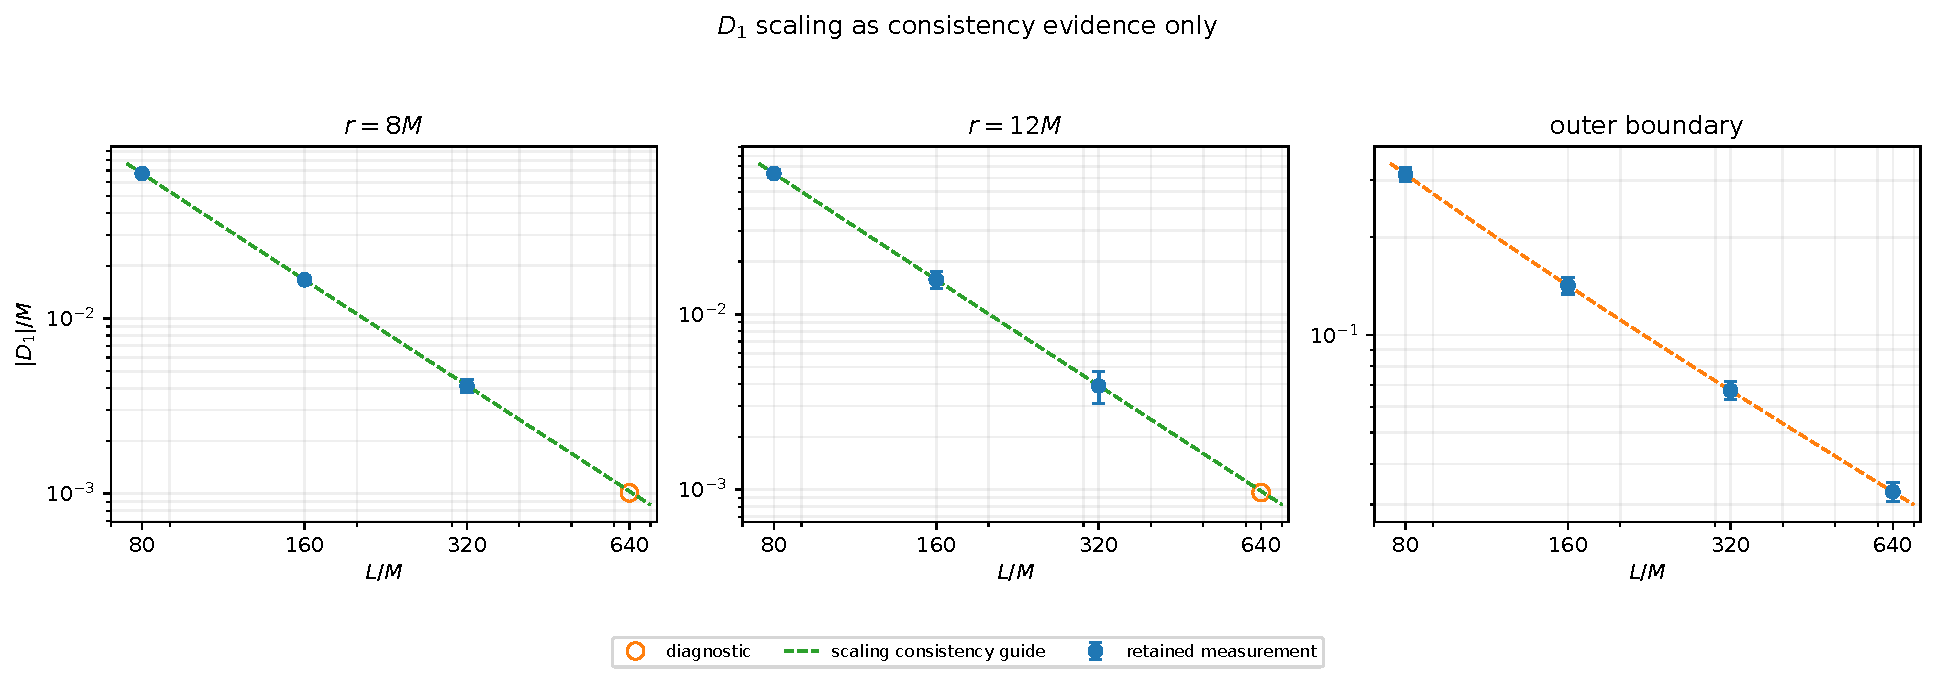
\includegraphics[width=\textwidth]{figs/D1_scaling.pdf}
 \caption{Minimally coupled ($\xi=0$) absolute shift $|D_1|$ in the
 direct-to-first-echo spacing at
 $r=8M$, $r=12M$, and the outer boundary.  Bars show combined deterministic
 sensitivities.  Open markers fail the $|D_1|\geq3\,\delta D_1$ selection
 condition.  Dashed curves show the sensitivity-weighted fits in
 Eq.~\eqref{eq:d1_scaling_models}.}
 \label{fig:d1}
\end{figure*}

\begin{figure*}[t]
 \centering
 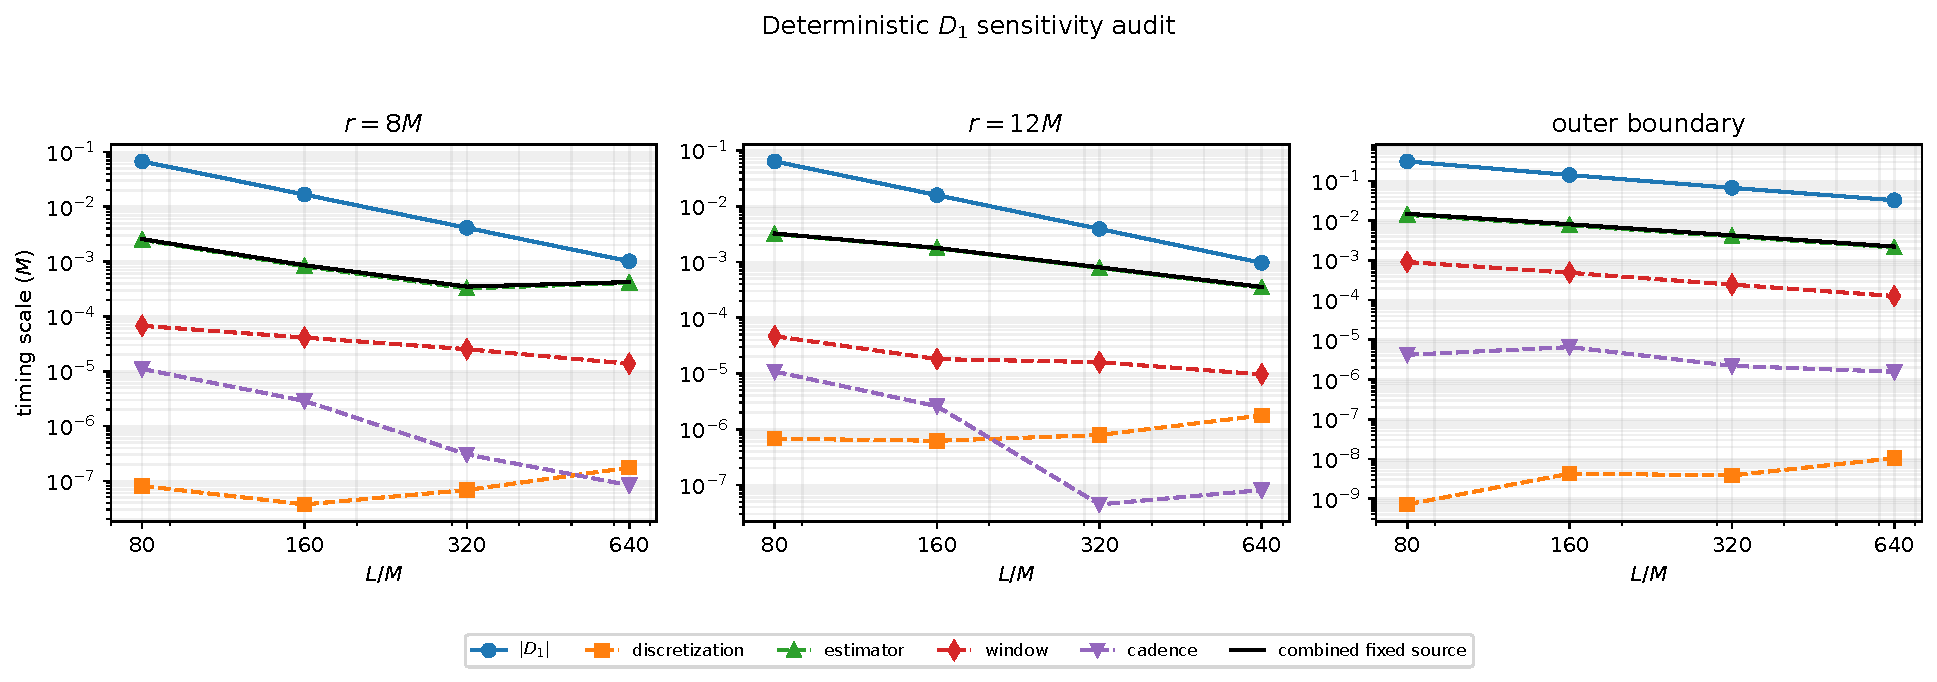
\includegraphics[width=\textwidth]{figs/D1_error_separation.pdf}
 \caption{Separation of the minimally coupled ($\xi=0$) deterministic
 $D_1$ sensitivities at each
 observer.  The measured $|D_1|$ is shown with the discretization,
 estimator, window, and cadence contributions and with their conservative
 linear sum.  The estimator contribution dominates the sum at every length,
 which is what prevents a precision coefficient statement.}
 \label{fig:d1_errors}
\end{figure*}

\clearpage
\begin{center}
\begin{minipage}{\columnwidth}
 \centering
 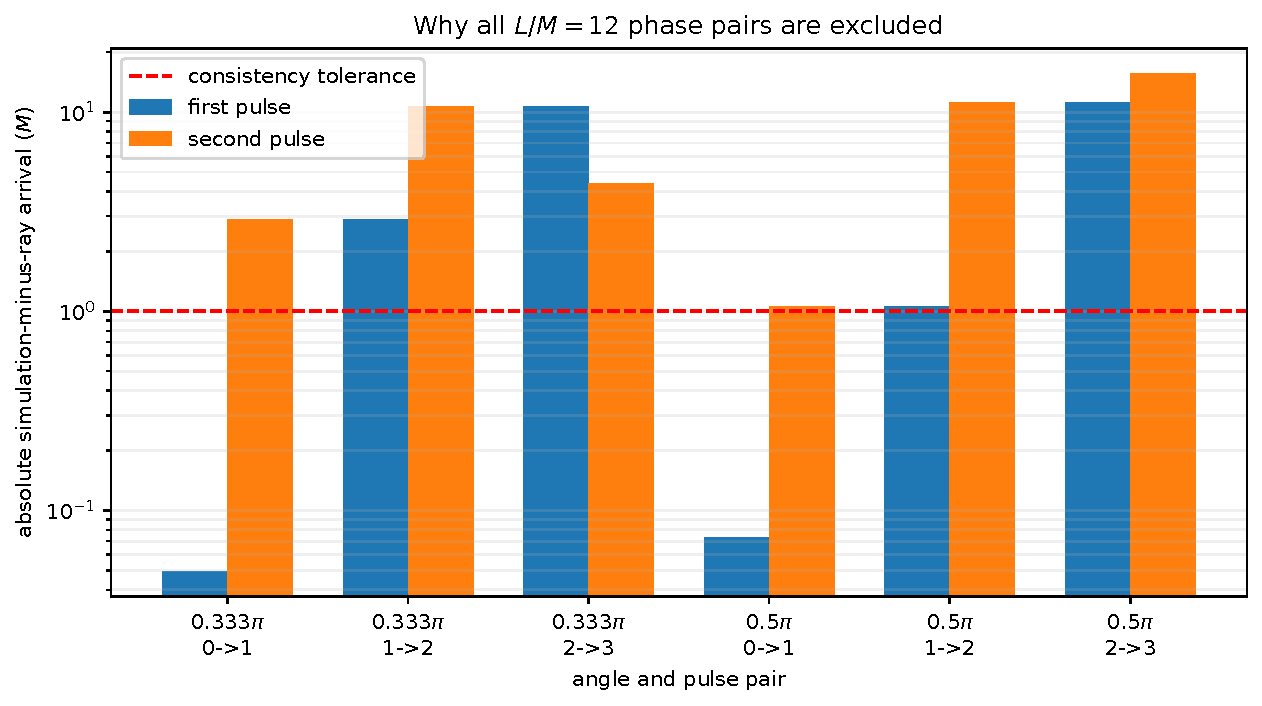
\includegraphics[width=\columnwidth]{figs/L12_phase_exclusion.pdf}
 \captionof{figure}{Null geodesic residuals of the extracted minimally coupled
 ($\xi=0$) pulses for the $L/M=12$ generic angle pairs.  Every pair has at least one pulse outside the
 declared $1M$ tolerance, so all six are excluded from quantitative phase
 analysis.}
 \label{fig:l12}
\end{minipage}
\end{center}

The checks above are what separate a reproducible measurement from a
resolved accuracy.  Refinement changes and Richardson estimates are reported
separately throughout, and the deterministic extraction sensitivities are
neither statistical standard deviations nor fit weights with a chi-squared
interpretation.

\clearpage
\section{Late-time departure and matched tail protocol}
\label{app:latetime}

The main text quotes the $\xi=0$, $r=8M$ transition because it is the cleanest
supporting case.  This separate crossover study treats the $\ell=1$ response
for $L/M=20$, $40$, $80$, and $160$ at $r=4M$, $8M$, $16M$, and $\hc$.
Finite-radius observations are compared with a separate Schwarzschild
run at the same areal radius, while $\hc$ is compared with Schwarzschild
$\scri^+$.  An additional $\ell=2$, $L/M=80$ calculation checks the
mode dependence.

Departure is the end of the last persistent interval, before cosmological
entry, on which the local decay rate agrees with the Schwarzschild reference.
Entry is the first persistent interval on which the rate agrees with the
expected minimally coupled SdS value.  The rate is constructed from a
centered root mean square
envelope and a cubic Savitzky--Golay filter.  We repeat the extraction for
$54$ combinations of smoothing width, root-mean-square fraction, persistence
interval, and tolerance.  A setting resolves a transition only when it finds
both endpoints.  At the aggregate level, a case is called resolved when at
least $27$ settings do so and marginal when between $1$ and $26$ do so.  If
none resolves, the case is reported by the missing endpoint, such as ``no
cosmological entry.''  Quoted times are medians over the resolving settings,
with the full sweep range as a systematic interval.

At $r=8M$, the entry medians are $\kappa_cU=2.83$ for $L/M=80$ and $2.94$
for $L/M=160$, with sweep ranges $[2.56,3.07]$ and $[2.68,3.19]$.
They agree to $4\%$ in cosmological units while the corresponding geometric
times differ by a factor of $2.05$.  The departure medians, $115.9M$ and
$133.5M$, are instead approximately fixed in black-hole units; their
dimensionless ranges are $[1.15,1.76]$ and $[0.71,0.96]$ in $\kappa_cU$.
The transition interval consequently widens from approximately $117M$ to
$343M$.  With only two clean lengths, this contrast is consistency evidence
for the two physical scales and not a fitted scaling law.

The shorter-length cases show why the aggregate classification matters.  At
$L/M=20$ no observer enters a resolved cosmological regime.  At $L/M=40$ the
$r=4M$ case has no cosmological entry, the $r=8M$ and $r=16M$ cases are
marginal with respectively $1/54$ and $18/54$ resolving settings, while the
cosmological-horizon case is resolved at the threshold $27/54$.

The Schwarzschild reference does not settle within $5\%$ of its own
$\ell=1$ Price value until $U=220.3M$ at $r=8M$ and $167.3M$ at $\scri^+$,
both later than the corresponding finite-$L$ departures.  For $\ell=2$ the
Price value is not attained at $r=4M$ within the evolved interval.  Thus the
tested finite-$L$ solutions leave the Schwarzschild waveform before a clean
Schwarzschild power-law regime is established.  This supplies physical
context for the finite-$L$ comparison interval; the production disjoint
windows in Sec.~\ref{sec:direct_recovery} are labeled diagnostic for the
separate numerical reason that their refinement change is not subdominant.

\subsection{Exterior-tail formulation check}
\label{app:tail-formulation-check}

The standard and shared-flux reductions are algebraically equivalent, but
the exterior-tail production calculation changes their semidiscrete form.
We therefore checked the waveform on the same exterior background rather
than relying on the continuum transformation alone.  A direct short
standard-versus-shared-flux regression at $L/M=80$ agrees in absolute
waveform amplitude to better than $10^{-7}$.  The long independent check uses
endpoint-factored fields
\begin{equation}
 H=\alpha_+(\pi+\psi),\qquad
 J=\alpha_-(\pi-\psi),
 \label{eq:factored_characteristics}
\end{equation}
so that the physical fluxes are $(1-\rho)H$ and $\rho J$.  It damps only the
continuum reduction constraint, for which
$\partial_\tau C=-M^{-1}C$, and evolves the same scalar equation, geometry,
initial data, clock, and output times as the shared-flux production system.

For $L/M=640$, $\ell=1$, and $\xi=0$, both formulations were evolved through
$U/M=1000$ at $N=1536$ and $2048$ with
$\Delta\tau/M=0.0025$.  At $N=2048$, their outer-boundary relative
$L^2$ differences range from $0.62\%$ to $2.65\%$ over six late-signal audit
windows between $U/M=100$ and $950$; the small late amplitude makes these
windowed relative differences more stringent than the prompt-dominated
full-record norm.  More importantly, the endpoint-factored and shared-flux
systems give longest $p_{\rm eff}\simeq3$ intervals of $12.15M$ and $11.90M$,
respectively.  Both independently fail the required $40M$ persistence test.
The former gives a median slow-component index $p_{\rm eff}=1.176$, while the
latter gives $p=1.086$ with $R^2=0.9926$ on its fixed $120$--$250M$ fit.
Thus the negative Price-law classification and the slow exterior component
do not arise from the shared-flux reduction.  This comparison is a
formulation check, not an additional accuracy estimate; the production
accuracy is set by the three-grid and halved-timestep ladders.

\subsection{Matched outer-boundary tail protocol}

The regulator question concerns radiation at the asymptotic end.  The
large-$L$ tail comparison therefore uses an $\ell=1$ waveform at $\hc$ for
uniform and exterior-supported SdS and compares it with the same Schwarzschild
waveform at $\scri^+$.  The completed calculation uses $L/M=640$ and extends
through $U/M=1000$ for both $\xi=0$ and $1/6$.  This test complements the
finite-radius crossover above: it asks whether a finite cosmological boundary
can reproduce even a short interval of the Schwarzschild null-infinity Price
law before its own asymptotics take over.

From a centered root-mean-square envelope $A(U)$ we form the local power index
$p_{\rm eff}=-d\ln A/d\ln U$.  A candidate Schwarzschild-like interval must
remain within $10\%$ of the null-infinity dipole value $p=3$ for at least
$40M$.  A candidate subsequent exponential regime is measured with
$\gamma_{\rm eff}=-d\ln A/dU$.  For uniform SdS, the large-$L$ reference rates are
$\gamma_{\rm eff}/\kappa_c\simeq1$ for $\xi=0$ and $2$ for $\xi=1/6$.
The uniform rate must remain within $10\%$ of its target for at least the
semilog fit width $\Delta(\kappa_cU)=0.25$.  No target is imposed on the
exterior-supported geometry; its late signal is analyzed without assigning
an asymptotic decay law.
Each claimed interval lies above the time-dependent numerical floor and
persists under an envelope- and fit-window sweep.  Three spatial resolutions
and a fixed-resolution halved-timestep run test the ordering and duration of
the intervals.  The primary estimator uses a $10M$ envelope and $40M$ local
fit.  We also combine envelope widths $5M$, $10M$, and $20M$ with fit widths
$30M$, $40M$, and $60M$.  Across these nine choices, the Schwarzschild
candidate lasts $815.4$--$841.9M$ and the uniform conformal candidate lasts
$131.1$--$148.1M$; both pass.  The longest candidates in uniform minimal,
exterior minimal, and exterior conformal SdS last at most $10.2M$, $12.0M$,
and $11.3M$, respectively, so all three fail.  The classification is therefore
insensitive to the estimator widths.

Figure~\ref{fig:matched-tail} and Table~\ref{tab:matched-tail} give the full
comparison.  The exterior features converge under refinement, but neither
coupling resolves a Schwarzschild Price interval or a cosmological entry.
These null results are retained rather than converted into crossover times.

\section{Reproducibility record}
\label{app:reproducibility}

The public reproducibility package separates the $36$ raw $\xi=0$ simulation
archives---$21$ for the fixed-mode family and $15$ for the localized-source
family---from all derived tables and figures.  Each archive records the
physical configuration, numerical resolution, generating command, software
version, and checksum.  A machine-readable manifest links every reported
artifact to its inputs and verifies that postprocessing leaves the raw
archives unchanged.
A unified exterior-QNM manifest covers the three Schwarzschild controls,
$12$ uniform-SdS controls, and $12$ exterior-supported archives and links all
$27$ waveform inputs to the reported residual figure and numerical table.
A separate matched tail package contains $20$ archives: three spatial grids
and one halved-timestep run for each of the Schwarzschild, uniform-minimal,
uniform-conformal, exterior-minimal, and exterior-conformal families.  Its
checksum index links the raw waveforms to the estimator sweep,
Table~\ref{tab:matched-tail}, and Fig.~\ref{fig:matched-tail}.  The older
Schwarzschild and uniform control archives store unused field snapshots on the
dealiased grid, whereas the repaired exterior archives store them on the base
grid.  The tail analysis uses only the identically sampled observer waveforms;
all are finite and pass their reduction-constraint checks.
The independent exterior formulation check adds two endpoint-factored
$L/M=640$, $\xi=0$ archives at $N=1536$ and $2048$.  They use the same
physical configuration and extend to the same final retarded time as the
corresponding shared-flux archives.

The physical contracts recorded with the two simulation families fix the
mass normalization, foliation and compactification, data or source
prescription, and waveform clock.  The release also includes the supporting
foliation-conditioning, late-time crossover, and cross-implementation data
used in the manuscript, together with the corresponding analysis scripts.
The compact encoding of the localized responses has a maximum relative peak
reconstruction error of $10^{-7}$, negligible for the percent-level waveform
comparisons.  Consequently, the small refinement values in
Table~\ref{tab:localized} are used only to establish that discretization is
subdominant, not to claim accuracy at the displayed digits.

\begin{acknowledgments}
A.Z. thanks Ted Jacobson, Rodrigo Panosso Macedo, and Alex
Va\~n\'o-Vi\~nuales for discussions.  This work was inspired by Charles
Misner's investigations of artificial cosmology and by the memorial
symposium held at the University of Maryland in 2023.  This material is
supported by NSF Grant No.~2309084.
\end{acknowledgments}

\section*{Data Availability}
The code, simulation data, and analysis scripts supporting this study are
publicly available in Ref.~\cite{blackhole_computation_2026}.

\bibliographystyle{apsrev4-2}
\makeatletter
\immediate\write\@auxout{\string\citation{apsrev42Control}}
\makeatother
\bibliography{SdS_refs}

\end{document}
